\documentclass[preprint,12pt]{elsarticle}
\usepackage[utf8]{inputenc}
\usepackage[T1]{fontenc}
\usepackage{amsmath,amssymb}
\usepackage{algorithm}
\usepackage{algpseudocode}
\usepackage{graphicx}
\usepackage{booktabs}
\usepackage{longtable}
\usepackage{array}
\usepackage{float}
\usepackage{calc}
\usepackage{etoolbox}
\AtBeginEnvironment{longtable}{\small}
\setlength{\LTleft}{0pt}
\setlength{\LTright}{0pt}
\usepackage{url}
\usepackage{needspace}
\usepackage[hidelinks]{hyperref}
\providecommand{\tightlist}{} % pandoc artifact; no-op
\newcounter{tabno}
\newcommand{\tabcaption}[1]{\par\needspace{9\baselineskip}\refstepcounter{tabno}\noindent\textbf{Table \thetabno:} #1\par\vspace{2pt}}
\journal{Expert Systems with Applications}
\begin{document}
\begin{frontmatter}
\title{Label-Efficient and Risk-Controlled Adaptation of AI-Forged Document Detectors under Generator Shift}
\author{Anonymous submission}
\address{Author names withheld for review}
\begin{abstract}
Generative image editing has made it possible to alter a single numeric field in a financial document in under a second, and detectors trained on traditional (e.g., Photoshop-based) forgeries are largely blind to such edits. Even a detector trained on one generative inpainter collapses when the underlying generator changes --- a \emph{generator shift}. In realistic banking deployments, collecting many labelled forgeries for every new generator is infeasible. We study \textbf{label-efficient adaptation} of an AI-forged document detector under generator shift, and we ask whether a small number of labelled target-generator samples is sufficient to recover localization performance without catastrophically forgetting previously seen generators. Using the AIForge-Doc benchmark (Gemini, Ideogram, GPT-Image-2), we show that: (i) a detector trained on Gemini collapses on unseen generators (IoU 0.052 on GPT-Image-2); (ii) few-shot fine-tuning recovers localization monotonically, reaching IoU 0.195 ± 0.037 with only 100 labelled target samples ($\approx$3.7× over zero-shot); (iii) training from scratch with the same 100 labels is substantially worse (IoU 0.085), showing that base-generator pretraining matters; and (iv) rehearsal of 100 old-generator samples restores in-domain performance to 0.672 ± 0.006 (near the 0.669 zero-shot level) at a modest target-generator cost (IoU 0.162). We further report a set of negative results: temperature scaling, global and per-image threshold calibration, sample-selection strategies, encoder freezing, frequency channels, and generic anomaly detection do \textbf{not} provide consistent gains. Our analysis indicates that the bottleneck is \textbf{localization precision}, not decision-threshold calibration. Finally, we show that adapting a native-resolution patch segmenter with the same 100 labels raises the localization ceiling from 0.459 to 0.677 IoU, but that the coarse peak used to position it is the real bottleneck: it misses the field centre by 152 px (median), so the crop covers only 53\% of the tampered pixels. Replacing the single peak with a dense high-resolution search over 384 px windows and selecting by patch confidence reaches \textbf{0.537 ± 0.016 IoU on the full unseen generator (2.8× the full-image baseline, 79\% of the adapted ceiling)}, and 0.284 IoU on a completely unseen generator (Ideogram) versus 0.114 for the full-image detector. A localization study shows that centroid, grid, zoom and tiling variants all underperform dense search, that the coarse map is too unreliable to prune it, and that the residual gap is a \emph{selection-confidence} problem under generator shift (oracle-window IoU is 0.653). We then state the guarantee where the signal lives: with 300 labelled documents, a split-conformal threshold controls the image-level miss rate at the nominal level (9.8\% at $\alpha=0.10$) but flags \textbf{55.8\% of authentic documents}, and the pixel-level miss rate saturates at \textbf{15.5\% at 5.5\% pixel false alarms} because the selected window misses part of the annotation in about 15\% of documents. Conformal risk control therefore gives a one-sided guarantee on misses, not a usable operating point: image triage remains the deployment bottleneck. We release code, splits, and all results for reproducibility.
\end{abstract}
\begin{keyword}
AI-forged documents \sep forgery localization \sep few-shot adaptation \sep generator shift \sep conformal risk control
\end{keyword}
\end{frontmatter}

\section{Introduction}\label{introduction}

Digital document fraud is increasing rapidly. Recent generative inpainting APIs can replace a number or a date in a photographed receipt while preserving font, colour, and texture, leaving no obvious compression or copy-move traces. Detectors designed for traditional document tampering therefore degrade substantially on such forgeries.

A second, less discussed problem is \textbf{generator shift}. A detector trained on forgeries produced by one inpainting model learns generator-specific artefacts rather than a generator-agnostic notion of tampering. When a new generator appears, the detector collapses. In a bank, this is operationally critical: the institution cannot wait to collect thousands of labelled forgeries for every new tool.

We therefore study a practical question:

\begin{quote}
\emph{Given a detector trained on an old generator, how many labelled samples from a new generator are needed to recover localization, and how can we adapt without forgetting the old generator?}
\end{quote}

We use the AIForge-Doc benchmark~\cite{wu2026aiforgedoc}, which provides AI-inpainted financial and form documents with pixel-precise masks for three generator families: Gemini 2.5 Flash Image, Ideogram v2 Edit, and GPT-Image-2~\cite{wu2026forgerjudge}. We adopt a leave-one-generator-out protocol and evaluate both localization (IoU/F1/Dice) and detection-oriented metrics (image AUC/AP, Recall@1\%FPR).

\textbf{Contributions.}

\begin{enumerate}
\def\labelenumi{\arabic{enumi}.}
\tightlist
\item
  A controlled study of label-efficient adaptation for AI-forged document detection under generator shift.
\item
  A few-shot adaptation curve (k = 0, 5, 25, 100; 3 seeds) showing monotonic recovery (IoU 0.052 -\textgreater{} 0.195 ± 0.037).
\item
  A rehearsal strategy that restores old-generator performance to near zero-shot level (Gemini IoU 0.672 ± 0.006) while retaining most of the adaptation gain.
\item
  An honest set of negative results: calibration, adaptive thresholding, sample selection, encoder freezing, frequency channels, and generic anomaly detection do not provide consistent gains; we analyze why.
\item
  Qualitative evidence (score maps) showing that adaptation sharpens localization rather than merely shifting thresholds.
\item
  A \textbf{text-localized high-resolution search (TL-HRS) method} that adapts a patch segmenter with the same 100 target labels and searches the document densely at native resolution: the localization ceiling rises from 0.459 to 0.677, and the automatic pipeline reaches \textbf{0.537 ± 0.016 IoU} on the full unseen generator (2.8× the full-image baseline, 79\% of the ceiling), while a single coarse peak reaches only 0.321.
\item
  A localization study showing that the coarse stage, not segmentation, is the bottleneck (median peak error 152 px; crop coverage 53\% vs.~98\% at the true box), and that dense search beats centroid refinement, grids, zoom, tiling, coarse-guided pruning, OCR selection, multi-signal fusion and pixel gating; the remaining gap is uncalibrated selection confidence under generator shift.
\item
  A \textbf{risk-controlled localization} analysis: with 300 labelled documents, split-conformal risk control holds for image-level misses (9.8\% at $\alpha=0.10$) but only at 55.8\% image false alarms, and pixel-level FNR saturates at 15.5\% (5.5\% pixel FPR) because of the window-miss floor. We report the guarantee as one-sided and identify image triage, not localization, as the remaining bottleneck.
\end{enumerate}

\bigskip

\section{Related Work}\label{related-work}

\textbf{AI-forged document detection.} DocTamper~\cite{qu2023doctamper} (CVPR 2023) introduced a large document-tampering benchmark and a document-specific detector built on compression-artifact tracing, later extended by CAT-Net~\cite{kwon2021catnet} and PSCC-Net~\cite{liu2022pscc}; MVSS-Net~\cite{chen2021mvss} and HiFi-Net~\cite{cao2022hifinet} approached the same problem with multi-view supervision and reconstruction-classification learning. On the general-image side, TruFor~\cite{guillaro2023trufor} combines a transformer backbone with a learned noise fingerprint, Noiseprint~\cite{cozzolino2019noiseprint} models camera fingerprints, and ManTra-Net~\cite{wang2019mantra} and RGB-N~\cite{zhou2018rgbn} exploit anomalous features and rich boundary cues. AIForge-Doc~\cite{wu2026aiforgedoc}, DOCFORGE-BENCH~\cite{zhao2026docforge} and the GPT-Image-2 study recently showed that all of these degrade severely on diffusion-inpainted documents, and that the problem remains open. Our work builds directly on AIForge-Doc and studies adaptation rather than zero-shot detection.

\textbf{Detection of generated content.} A parallel literature asks whether an image was generated at all, using frequency cues, diffusion reconstruction error (DIRE)~\cite{wang2023dire}, or learned fingerprints. These detectors operate at image level and assume a globally synthetic image; our target is a small inpainted region inside an otherwise authentic financial document, which is why image-level scores are weak here and why the guarantee must be stated at the localization level.

\textbf{High-resolution and coarse-to-fine localization.} Patch-based and coarse-to-fine pipelines are standard in segmentation and in forgery localization, typically using a low-resolution proposal followed by a native-resolution crop. We show that the proposal stage is the bottleneck for thin, wide text fields: the coarse peak misses the field centre by 152 px (median), so we replace it with a dense high-resolution search scored by patch confidence. This connects to sliding-window detection and to cascade designs that trade compute for accuracy.

\textbf{Few-shot and continual adaptation.} Few-shot learning (MAML~\cite{finn2017maml}, Prototypical Networks~\cite{snell2017proto}) and unsupervised domain adaptation are mature. We do not propose a new adaptation algorithm; instead we characterize how standard fine-tuning behaves under extreme label scarcity and generator shift. Rehearsal (experience replay)~\cite{rolnick2019replay} is the classical remedy for catastrophic forgetting, with EWC~\cite{kirkpatrick2017ewc}, LwF~\cite{li2017lwf}, iCaRL~\cite{rebuffi2017icarl}, A-GEM~\cite{chaudhry2019agem} and DER++~\cite{buzzega2020der} as the main representatives; we show that a 100-sample replay buffer is enough, and that at the patch level replay acts as additional data rather than as a pure anti-forgetting device.

\textbf{Calibration and distribution-free guarantees.} Temperature scaling~\cite{guo2017calibration} and Bayesian binning~\cite{naeini2015bbq} are standard post-hoc calibrators; we find they change confidence but not ranking. Conformal prediction~\cite{vovk2005conformal} and conformal risk control~\cite{angelopoulos2024crc,bates2021risk} provide distribution-free guarantees under exchangeability. We apply document-level CRC to image triage and to pixel-level false-negative control, and we report where exchangeability breaks under generator shift instead of claiming a guarantee that does not hold.

\section{Dataset and Protocol}\label{dataset-and-protocol}

\subsection{Dataset}\label{dataset}

We use \textbf{AIForge-Doc} (v1 and v2); Table~\ref{tab:dataset} lists the splits.

{
\tabcaption{AIForge-Doc splits used in this paper (forged/authentic pairs).}\label{tab:dataset}
\begin{longtable}[]{@{}llll@{}}
\toprule\noalign{}
Split & Forged & Authentic & Generators \\
\midrule\noalign{}
\endhead
\bottomrule\noalign{}
\endlastfoot
v1 train & 3,249 & 3,249 & Gemini (2,912), Ideogram (337) \\
v1 test & 812 & 812 & Gemini (727), Ideogram (85) \\
v2 train & 2,453 & 2,453 & GPT-Image-2 \\
v2 test & 613 & 613 & GPT-Image-2 \\
\end{longtable}
}

v1 and v2 pair each forged document with an authentic counterpart, so the authentic counts mirror the forged counts (v2 authentic pairs are used for adaptation and image-level evaluation). Documents are receipts and forms; forgeries replace a single numeric field. The median tampered area is $\approx$1\% of the image. Masks are binary (0/255). We verified the integrity of all 18,315 files (0 corrupt) and visually confirmed mask alignment.

\subsection{Leave-one-generator-out protocol}\label{leave-one-generator-out-protocol}

We define three settings:

\begin{itemize}
\tightlist
\item
  \textbf{P1 (zero-shot shift):} train on Gemini, test on Gemini (in-domain), Ideogram, and GPT-Image-2.
\item
  \textbf{P2:} train on Gemini + Ideogram, test on GPT-Image-2 (unseen).
\item
  \textbf{P3:} train on Gemini + GPT-Image-2, test on Ideogram (unseen).
\end{itemize}

Unless stated otherwise, the base detector is trained on Gemini (2,912 forged + 2,912 authentic).

\subsection{Metrics}\label{metrics}

\begin{itemize}
\tightlist
\item
  \textbf{Localization:} IoU, F1, Dice at threshold 0.5.
\item
  \textbf{Ranking:} pixel AUC (mean per image) and image AUC.
\item
  \textbf{Detection under alert budget:} image Average Precision (AP) and Recall at FPR = 1\% (Recall@1\%FPR), which reflects a bank's limited review capacity.
\end{itemize}

\subsection{Threat model}\label{threat-model}

The asset is a financial document whose numeric field has been replaced by a generative editor. The adversary wants to (i) evade image-level triage, (ii) displace or shrink the predicted mask so that a human reviewer cannot find the edit, or (iii) trigger false alarms on genuine documents. We assume a black-box adversary who can (a) use a generator not seen in training, (b) post-process the final document with operations that preserve legibility---JPEG recompression at messenger or bank settings, resizing, and mild blur---and (c) query the deployed system only through its output. White-box adversarial perturbations, physical recapture, whole-document synthesis, and collusion with the reviewer are out of scope. The model is deliberately modest: it captures the shift that occurs when a forger uses a new tool or sends the file through a messaging pipeline, which is exactly where the detectors above fail. Section~\ref{robustness-to-post-processing} quantifies the post-processing component.

\bigskip

\section{Method}\label{method}

Figure~\ref{fig:pipeline} gives an overview of TL-HRS: a coarse patch scan proposes windows, a local refinement selects $w^*$, and the adapted patch segmenter produces the mask. The same score $S(w)$ drives image-level triage, and the mask supports pixel-level risk control.

\begin{figure}[htbp]
\centering
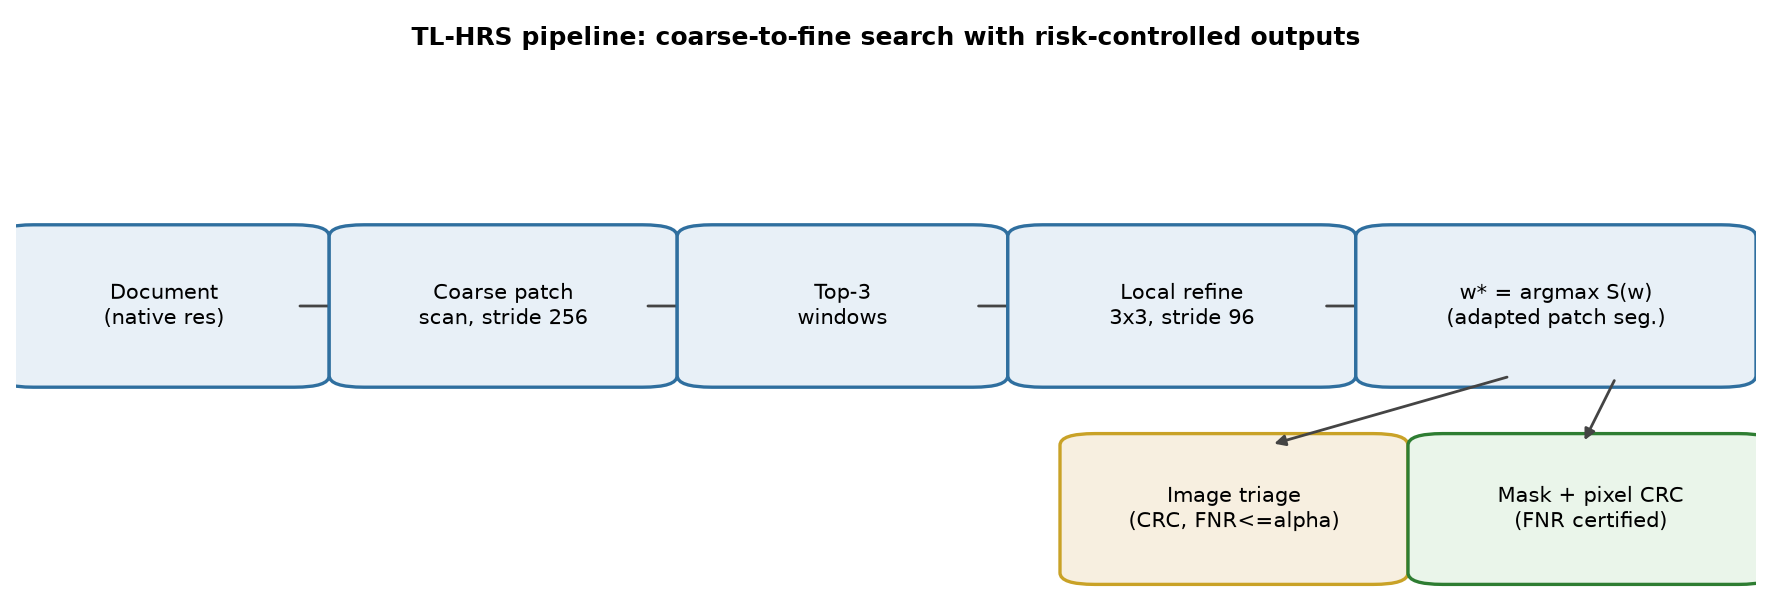
\includegraphics[width=\textwidth,keepaspectratio]{figures/fig_pipeline.png}
\caption{Overview of TL-HRS: a coarse patch scan proposes windows, a local refinement selects $w^*$, and the adapted patch segmenter produces the mask. The same score $S(w)$ drives image-level triage, and the mask supports pixel-level risk control.}
\label{fig:pipeline}
\end{figure}

\subsection{Base detector}\label{base-detector}

We use a U-Net~\cite{ronneberger2015unet} with a ResNet-18 encoder~\cite{he2016resnet} pretrained on ImageNet. The model outputs a single-channel logit map. It is trained on Gemini with:
\begin{equation*}
\mathcal{L} = \mathrm{BCEWithLogits}(\hat{y}, y; w{=}20) + \mathcal{L}_{\mathrm{Dice}},
\end{equation*}
where the positive weight compensates for the extreme pixel imbalance ($\approx$1\% tampered). Inputs are letterboxed to $384\times384$ to preserve document aspect ratio. Training uses AdamW (learning rate $10^{-4}$) for 10 epochs.

\subsection{Few-shot adaptation}\label{few-shot-adaptation}

Given k labelled samples from the target generator (plus k authentic samples), we fine-tune the base detector for 10 epochs with the same loss and optimizer. All models are evaluated on a disjoint target test split.

\subsection{Rehearsal}\label{rehearsal}

To mitigate forgetting, we add r samples from the old generator (Gemini) to the fine-tuning set. We compare random replay with two informed selectors: \textbf{hard} (highest per-sample BCE under the base model) and \textbf{uncertainty} (highest predictive entropy).

\subsection{Calibration (studied as an ablation)}\label{calibration-studied-as-an-ablation}

We study three calibration strategies: temperature scaling fitted on a held-out fraction of the labelled target samples; global threshold optimization; and per-image adaptive thresholding (keep the top-p\% pixels). These are evaluated but, as shown in Section 6.5, do not provide consistent gains.

\subsection{Text-localized high-resolution search (TL-HRS)}\label{text-localized-high-resolution-search-tl-hrs}

Algorithm~\ref{alg:tlhrs} summarises the procedure; $\lambda_{\mathrm{CRC}}(\alpha)$ is calibrated on the $n_{\mathrm{cal}}$ labelled documents as described in Section 6.13.

\begin{algorithm}[htbp]
\caption{TL-HRS with risk control}
\label{alg:tlhrs}
\begin{algorithmic}[1]
\Require document $x$, patch segmenter $f_\theta$, strides $s_1{=}256$, $s_2{=}96$, risk level $\alpha$
\Ensure mask $m$, image score $s^*$, window $w^*$
\State $W \gets \{\text{windows centred at }(s_1 i,\, s_1 j)\}$
\State score each $w\in W$ by $S(w)=\text{mean of top-1\% of } f_\theta(x_w)$
\State $C \gets$ top-3 windows of $W$
\State $R \gets$ union of $3\times3$ neighbourhoods of $C$ at stride $s_2$
\State $w^* \gets \arg\max_{w\in R} S(w)$
\State $p \gets f_\theta(x_{w^*})$; \quad $m \gets p > 0.5$
\State $s^* \gets S(w^*)$; \quad flag forged if $s^* > \lambda_{\mathrm{CRC}}(\alpha)$
\State \Return $m,\, s^*,\, w^*$
\end{algorithmic}
\end{algorithm}

Full-image inference runs at a letterboxed 384×384, where the median tampered field ($\approx$148 px wide) occupies only a few pixels; the resulting mask is spatially imprecise. TL-HRS adds a native-resolution stage on top of the adapted detector.

\textbf{Patch adaptation.} A patch segmenter (the same U-Net, applied to $384\times384$ crops at native scale) is fine-tuned with the \emph{same} $k$ target labels: $k$ crops centred on the ground-truth fields, $k$ non-overlapping same-line negatives, $k$ authentic crops, plus $r$ replay crops from the old generator. Crop boxes are derived from the training masks by connected components, so no extra annotation is required. Formally, for a crop $x_w$ centred at window $w$ the model outputs logits $f_\theta(x_w)$ and probabilities $\hat{y}_w=\sigma(f_\theta(x_w))$.

\textbf{Dense search.} At inference we slide the crop over the document at stride $s$ and score every window by the mean of its top-1\% pixels,
\begin{equation*}
S(w) = \frac{1}{|P_{1\%}(w)|}\sum_{p\in P_{1\%}(w)} \hat{y}_w(p),
\qquad
w^* = \arg\max_{w\in\mathcal{W}} S(w),
\end{equation*}
where $P_{1\%}(w)$ is the set of the highest-probability 1\% pixels in window $w$ and $\mathcal{W}$ is the set of valid windows (stride $s=96$, $\approx$197 windows per forged document). The prediction is the thresholded patch probability map at $w^*$; no OCR, selector, gating or multi-scale fusion is used. The mean of the top 1\% is robust to the large background area and rewards windows that contain a sharp, high-confidence mask rather than merely a large low-confidence blob. The whole pipeline is offline-friendly ($\approx$20 s per document on one consumer GPU) and is evaluated end-to-end in Section 6.8.

\bigskip

\section{Experimental Setup}\label{experimental-setup}

\begin{itemize}
\tightlist
\item
  \textbf{Base training:} Gemini train split, 384×384, 10 epochs.
\item
  \textbf{Adaptation:} $k\in\{5,25,100\}$ forged + $k$ authentic target samples, 10 epochs.
\item
  \textbf{Rehearsal:} r = 100 old-generator samples.
\item
  \textbf{Seeds:} 3 seeds for the adaptation curve, 4 for rehearsal.
\item
  \textbf{Hardware:} a single NVIDIA RTX 5060 Laptop GPU (8 GB).
\item
  \textbf{Reproducibility:} fixed splits, seeds, and scripts are released.
\end{itemize}

\bigskip

\section{Results}\label{results}

\subsection{Zero-shot detector collapses under generator shift}\label{zero-shot-detector-collapses-under-generator-shift}

{
\tabcaption{Zero-shot detector performance under generator shift (trained on Gemini).}\label{tab:zero-shot}
\begin{longtable}[]{@{}lllllll@{}}
\toprule\noalign{}
Test set & IoU & F1 & Dice & Image AUC & Image AP & Recall@1\%FPR \\
\midrule\noalign{}
\endhead
\bottomrule\noalign{}
\endlastfoot
Gemini (in-domain) & 0.669 & 0.802 & 0.719 & 0.913 & 0.925 & 0.553 \\
Ideogram (unseen) & 0.098 & 0.179 & 0.109 & 0.559 & 0.559 & 0.038 \\
GPT-Image-2 (unseen) & 0.052 & 0.099 & 0.104 & 0.526 & 0.547 & 0.015 \\
\end{longtable}
}

Table~\ref{tab:zero-shot} reports the zero-shot results. A detector trained on Gemini achieves strong in-domain localization but collapses on unseen generators. Notably, on GPT-Image-2 the \emph{image-level} AUC is near chance, yet the \textbf{pixel AUC remains 0.899} (Section 6.5). In other words, the model still ranks tampered pixels above background, but its predicted mask is spatially imprecise. The image-level scores (top-1\% mean probability) confirm the same picture: Recall@1\%FPR falls from 0.553 in-domain to 0.015 on GPT-Image-2, so a bank operating at a 1\% alert budget would miss almost every unseen-generator forgery --- a strong argument for the localization-assisted review pipeline studied in Section 6.8.

\subsection{Few-shot adaptation recovers localization}\label{few-shot-adaptation-recovers-localization}

Table~\ref{tab:fewshot} reports localization and forgetting under the four label budgets.

{
\tabcaption{Few-shot adaptation on GPT-Image-2: localization and forgetting versus the number of labelled target samples $k$ (mean $\pm$ std over 3 seeds).}\label{tab:fewshot}
\begin{longtable}[]{@{}llllll@{}}
\toprule\noalign{}

k
 & 
IoU
 & 
F1
 & 
Dice
 & 
Pixel AUC
 & 
Gemini IoU (forgetting)
 \\
\midrule\noalign{}
\endhead
\bottomrule\noalign{}
\endlastfoot
0 & 0.052 & 0.099 & 0.104 & 0.899 & 0.669 \\
5 & 0.068 ± 0.015 & 0.126 ± 0.026 & 0.116 ± 0.020 & 0.877 ± 0.020 & 0.624 ± 0.017 \\
25 & 0.105 ± 0.031 & 0.189 ± 0.052 & 0.140 ± 0.040 & 0.830 ± 0.023 & 0.577 ± 0.031 \\
100 & \textbf{0.195 ± 0.037} & \textbf{0.325 ± 0.051} & \textbf{0.228 ± 0.022} & \textbf{0.907 ± 0.031} & \textbf{0.494 ± 0.054} \\
\end{longtable}
}

Image-level detection under the same label budgets (GPT-Image-2, 613 forged + 613 authentic; score = top-1\% mean probability; Table~\ref{tab:image-level}):

{
\tabcaption{Image-level detection on GPT-Image-2 under the same label budgets (613 forged + 613 authentic).}\label{tab:image-level}
\begin{longtable}[]{@{}llll@{}}
\toprule\noalign{}
k & Image AUC & Image AP & Recall@1\%FPR \\
\midrule\noalign{}
\endhead
\bottomrule\noalign{}
\endlastfoot
0 & 0.526 & 0.547 & 0.015 \\
5 & 0.529 ± 0.012 & 0.522 ± 0.010 & 0.014 ± 0.001 \\
25 & 0.515 ± 0.024 & 0.518 ± 0.021 & 0.019 ± 0.006 \\
100 & 0.565 ± 0.024 & 0.582 ± 0.016 & 0.042 ± 0.012 \\
\end{longtable}
}

Image-level discrimination improves with labels but remains weak at a 1\% alert budget; this is expected, since the target quantity is a small localized edit rather than a global texture change, and it motivates localization-assisted review rather than a pure image-level triage.

Adaptation improves localization monotonically, reaching a \textbf{3.7$\times$} IoU gain with only 100 labelled target samples. The cost is forgetting: in-domain Gemini drops from 0.669 to 0.494. Figure~\ref{fig:main}(a) visualizes the curve; Figure~\ref{fig:main}(b) compares standard fine-tuning, rehearsal, and training from scratch at $k=100$.

\begin{figure}[htbp]
\centering
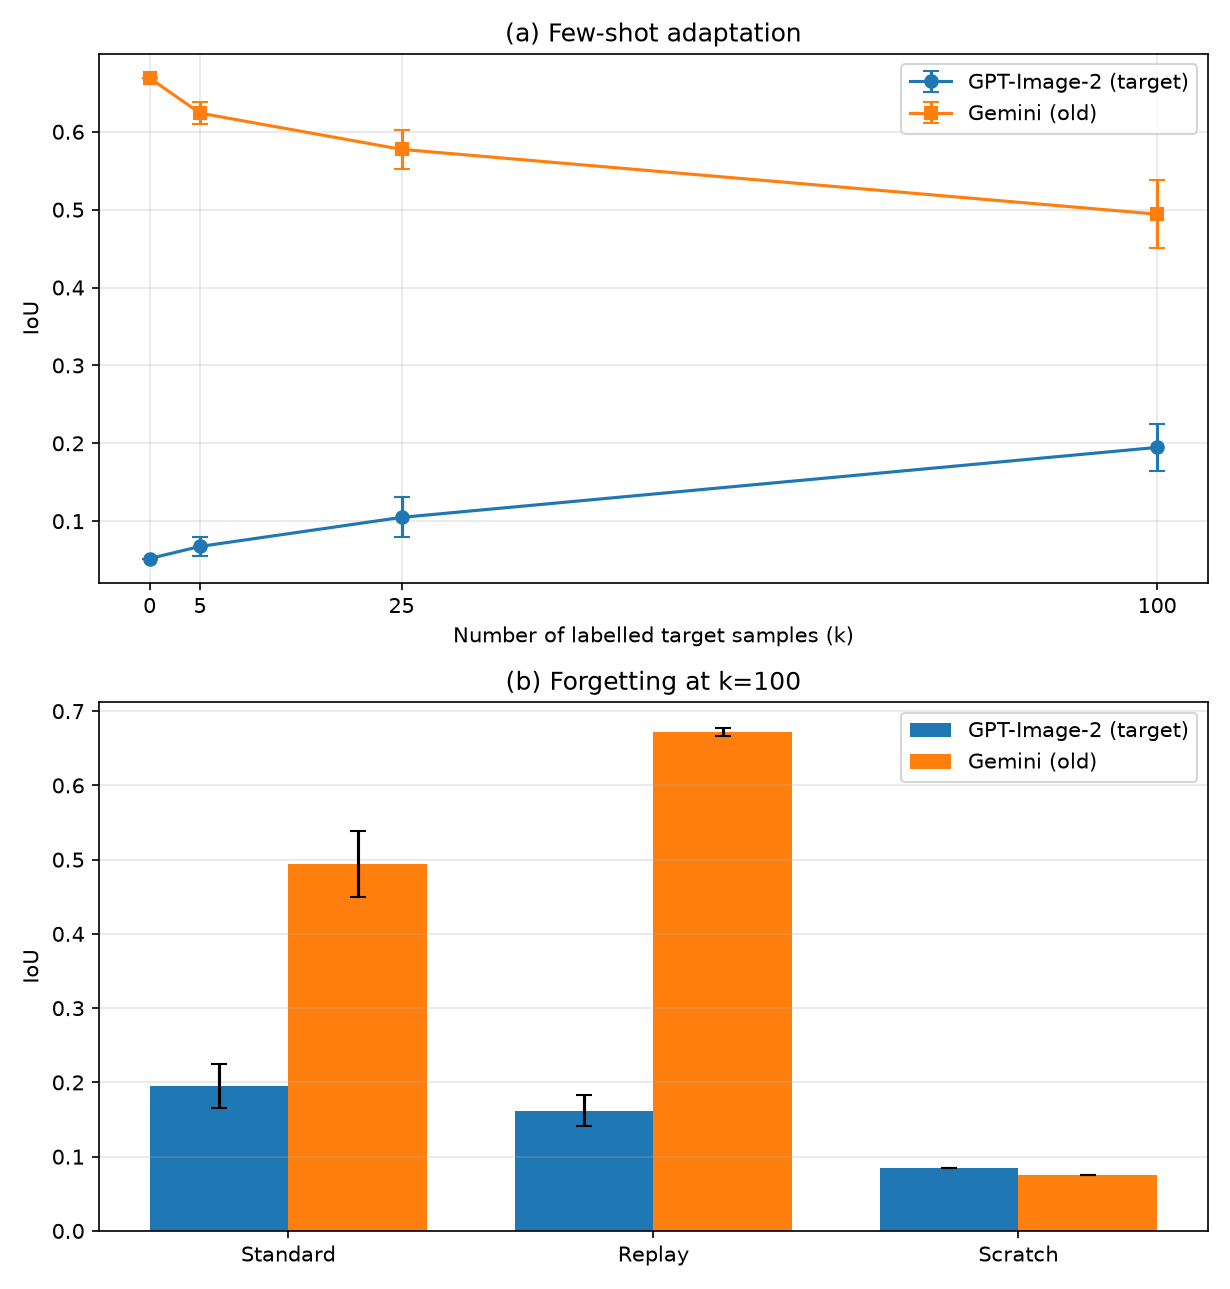
\includegraphics[width=\textwidth,keepaspectratio]{figures/fig_main_results.png}
\caption{(a)~Few-shot adaptation curve: IoU on the unseen GPT-Image-2 generator and on the old Gemini generator as a function of the number of labelled target samples (mean $\pm$ std over seeds). (b)~Forgetting at $k=100$: standard fine-tuning vs.~rehearsal vs.~training from scratch.}
\label{fig:main}
\end{figure}

\subsection{Pretraining matters: fine-tuning vs.~training from scratch}\label{pretraining-matters-fine-tuning-vs.-training-from-scratch}

{
\tabcaption{Fine-tuning from the Gemini base versus training from scratch with the same 100 labels.}\label{tab:scratch}
\begin{longtable}[]{@{}lllll@{}}
\toprule\noalign{}

Setting (k=100)
 & 
GPT IoU
 & 
GPT F1
 & 
Pixel AUC
 & 
Gemini IoU
 \\
\midrule\noalign{}
\endhead
\bottomrule\noalign{}
\endlastfoot
Fine-tune from Gemini base & \textbf{0.1597} & \textbf{0.2754} & \textbf{0.8536} & \textbf{0.5522} \\
Train from scratch & 0.0850 & 0.1567 & 0.6977 & 0.0750 \\
\end{longtable}
}

Table~\ref{tab:scratch} shows that fine-tuning is $\approx$1.9$\times$ better than training from scratch on the target generator, and preserves old-generator knowledge far better. Label-efficient adaptation therefore benefits from base-generator pretraining.

\subsection{Rehearsal eliminates forgetting}\label{rehearsal-eliminates-forgetting}

{
\tabcaption{Rehearsal at $k=100$: target adaptation and source retention.}\label{tab:rehearsal}
\begin{longtable}[]{@{}llll@{}}
\toprule\noalign{}

Method (k=100)
 & 
GPT IoU
 & 
Gemini IoU
 & 
Ideogram IoU
 \\
\midrule\noalign{}
\endhead
\bottomrule\noalign{}
\endlastfoot
Standard fine-tune (3 seeds) & 0.195 ± 0.037 & 0.494 ± 0.044 & 0.096 ± 0.014 \\
\textbf{Replay 100 (4 seeds)} & \textbf{0.162 ± 0.021} & \textbf{0.672 ± 0.006} & 0.108 ± 0.015 \\
\end{longtable}
}

Table~\ref{tab:rehearsal} shows that replay restores Gemini to \textbf{0.672 ± 0.006}, essentially the zero-shot level (0.669), at a modest target-generator cost (0.195 -\textgreater{} 0.162). This is the central practical finding: a small rehearsal buffer is sufficient to prevent catastrophic forgetting under generator shift.

Random replay performed best among the selectors; hard and uncertainty-based replay did not improve retention at the same budget.

\subsection{Negative results and ablations}\label{negative-results-and-ablations}

Table~\ref{tab:negative} summarises the ablations.

{
\tabcaption{Negative results and ablations (GPT-Image-2 target, Gemini source).}\label{tab:negative}
\begin{longtable}[]{@{}>{\raggedright\arraybackslash}p{0.25\linewidth}>{\raggedright\arraybackslash}p{0.29\linewidth}>{\raggedright\arraybackslash}p{0.16\linewidth}>{\raggedright\arraybackslash}p{0.22\linewidth}@{}}
\toprule\noalign{}
Strategy & Target (GPT) IoU & Old (Gemini) IoU & Conclusion \\
\midrule\noalign{}
\endhead
\bottomrule\noalign{}
\endlastfoot
Global threshold tuning & 0.160 $\rightarrow$ 0.194 (one model) & --- & modest, generator-specific \\
Temperature scaling & unchanged & unchanged & changes confidence, not ranking \\
Per-image adaptive threshold & 0.158 $\rightarrow$ 0.141 (p1\%) & 0.555 $\rightarrow$ 0.365 & worse than fixed 0.5 \\
Sample selection ($k{=}50$) & random 0.157; k-center 0.134; uncertainty 0.126 & --- & random is a strong baseline \\
Freeze encoder & 0.113 & 0.087 & fails \\
Augmentation (JPEG/blur/noise) & 0.052 $\rightarrow$ 0.054 & 0.669 $\rightarrow$ 0.589 & marginal, harms in-domain \\
Multi-generator training & P2 GPT 0.058; P3 Ideogram 0.121 & --- & marginal \\
Frequency channels (FR-Net) & 0.061 & 0.561 & marginal, harms in-domain \\
PatchCore~\cite{roth2022patchcore} (ResNet-18 / DINOv2~\cite{oquab2024dinov2}) & $\approx$0.05 (image AUC $\approx$0.5) & --- & fails \\
\end{longtable}
}

\textbf{Key observation.} Pixel AUC is consistently high (0.83--0.91) even when IoU is low, and neither temperature scaling nor per-image adaptive thresholding improves IoU. The bottleneck is therefore \textbf{spatial localization precision}, not decision-threshold calibration. This also explains why calibration tuned on the target generator can \emph{hurt} the old generator: it is generator-specific.

\subsection{Qualitative analysis}\label{qualitative-analysis}

Figure~\ref{fig:qual} shows score maps for the same forged GPT-Image-2 documents under three settings. Zero-shot predictions (Fig.~\ref{fig:qual}a) are diffuse, often off-target, and sometimes nearly blank. After adaptation (Fig.~\ref{fig:qual}b), score maps concentrate on the edited field. In-domain maps (Fig.~\ref{fig:qual}c) are sharp and closely match the ground truth. The qualitative evolution mirrors the quantitative gains.

\begin{figure}[htbp]
\centering
\begin{minipage}[t]{0.31\textwidth}\centering
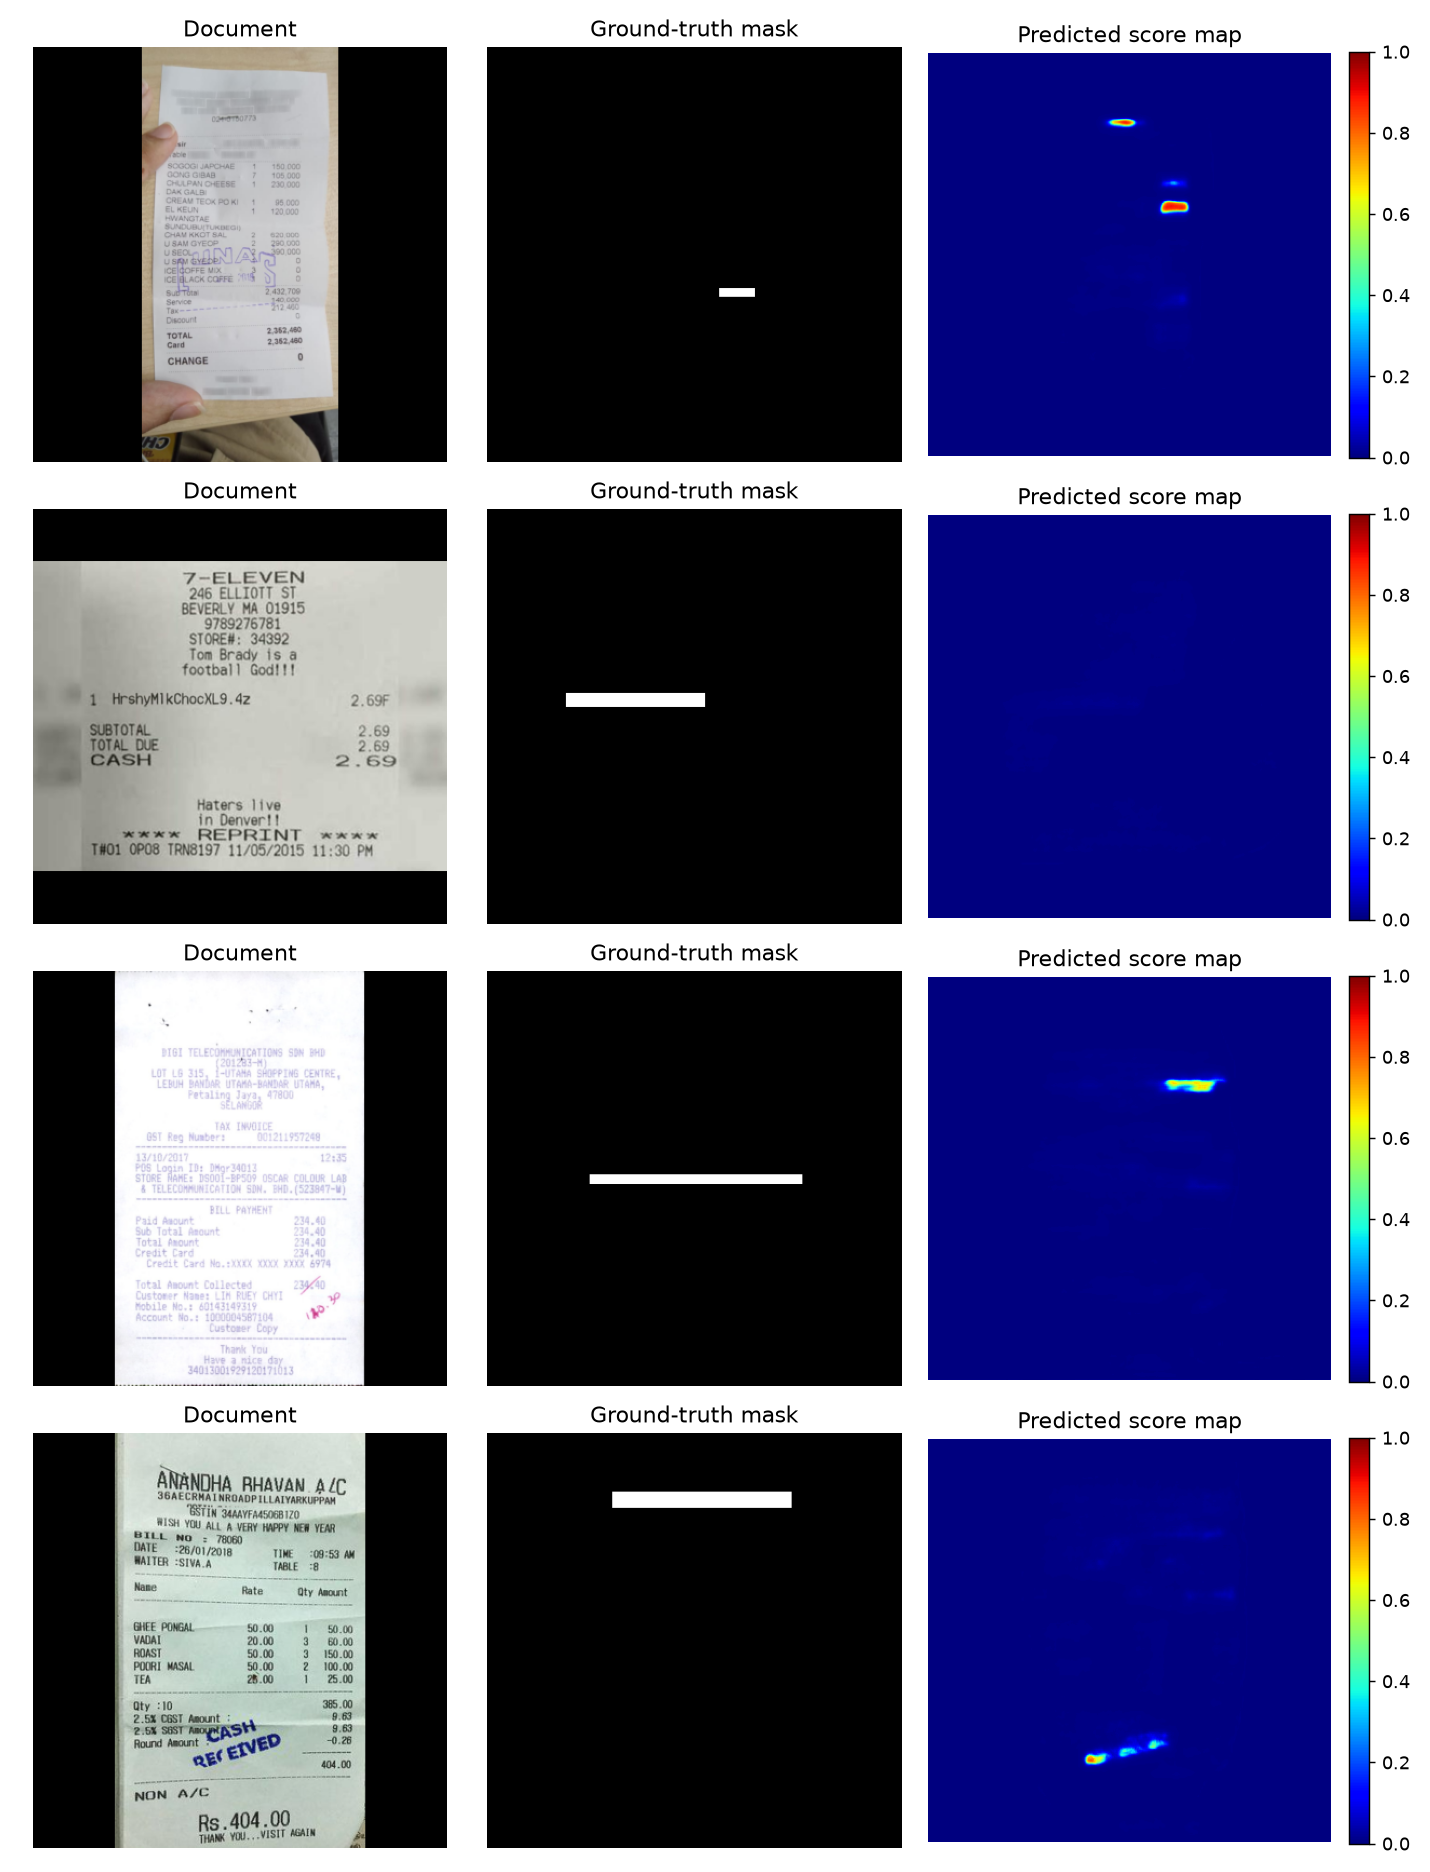
\includegraphics[width=\linewidth,keepaspectratio]{figures/fig_xai_zero_shot_gpt.png}\\(a)
\end{minipage}\hfill
\begin{minipage}[t]{0.31\textwidth}\centering
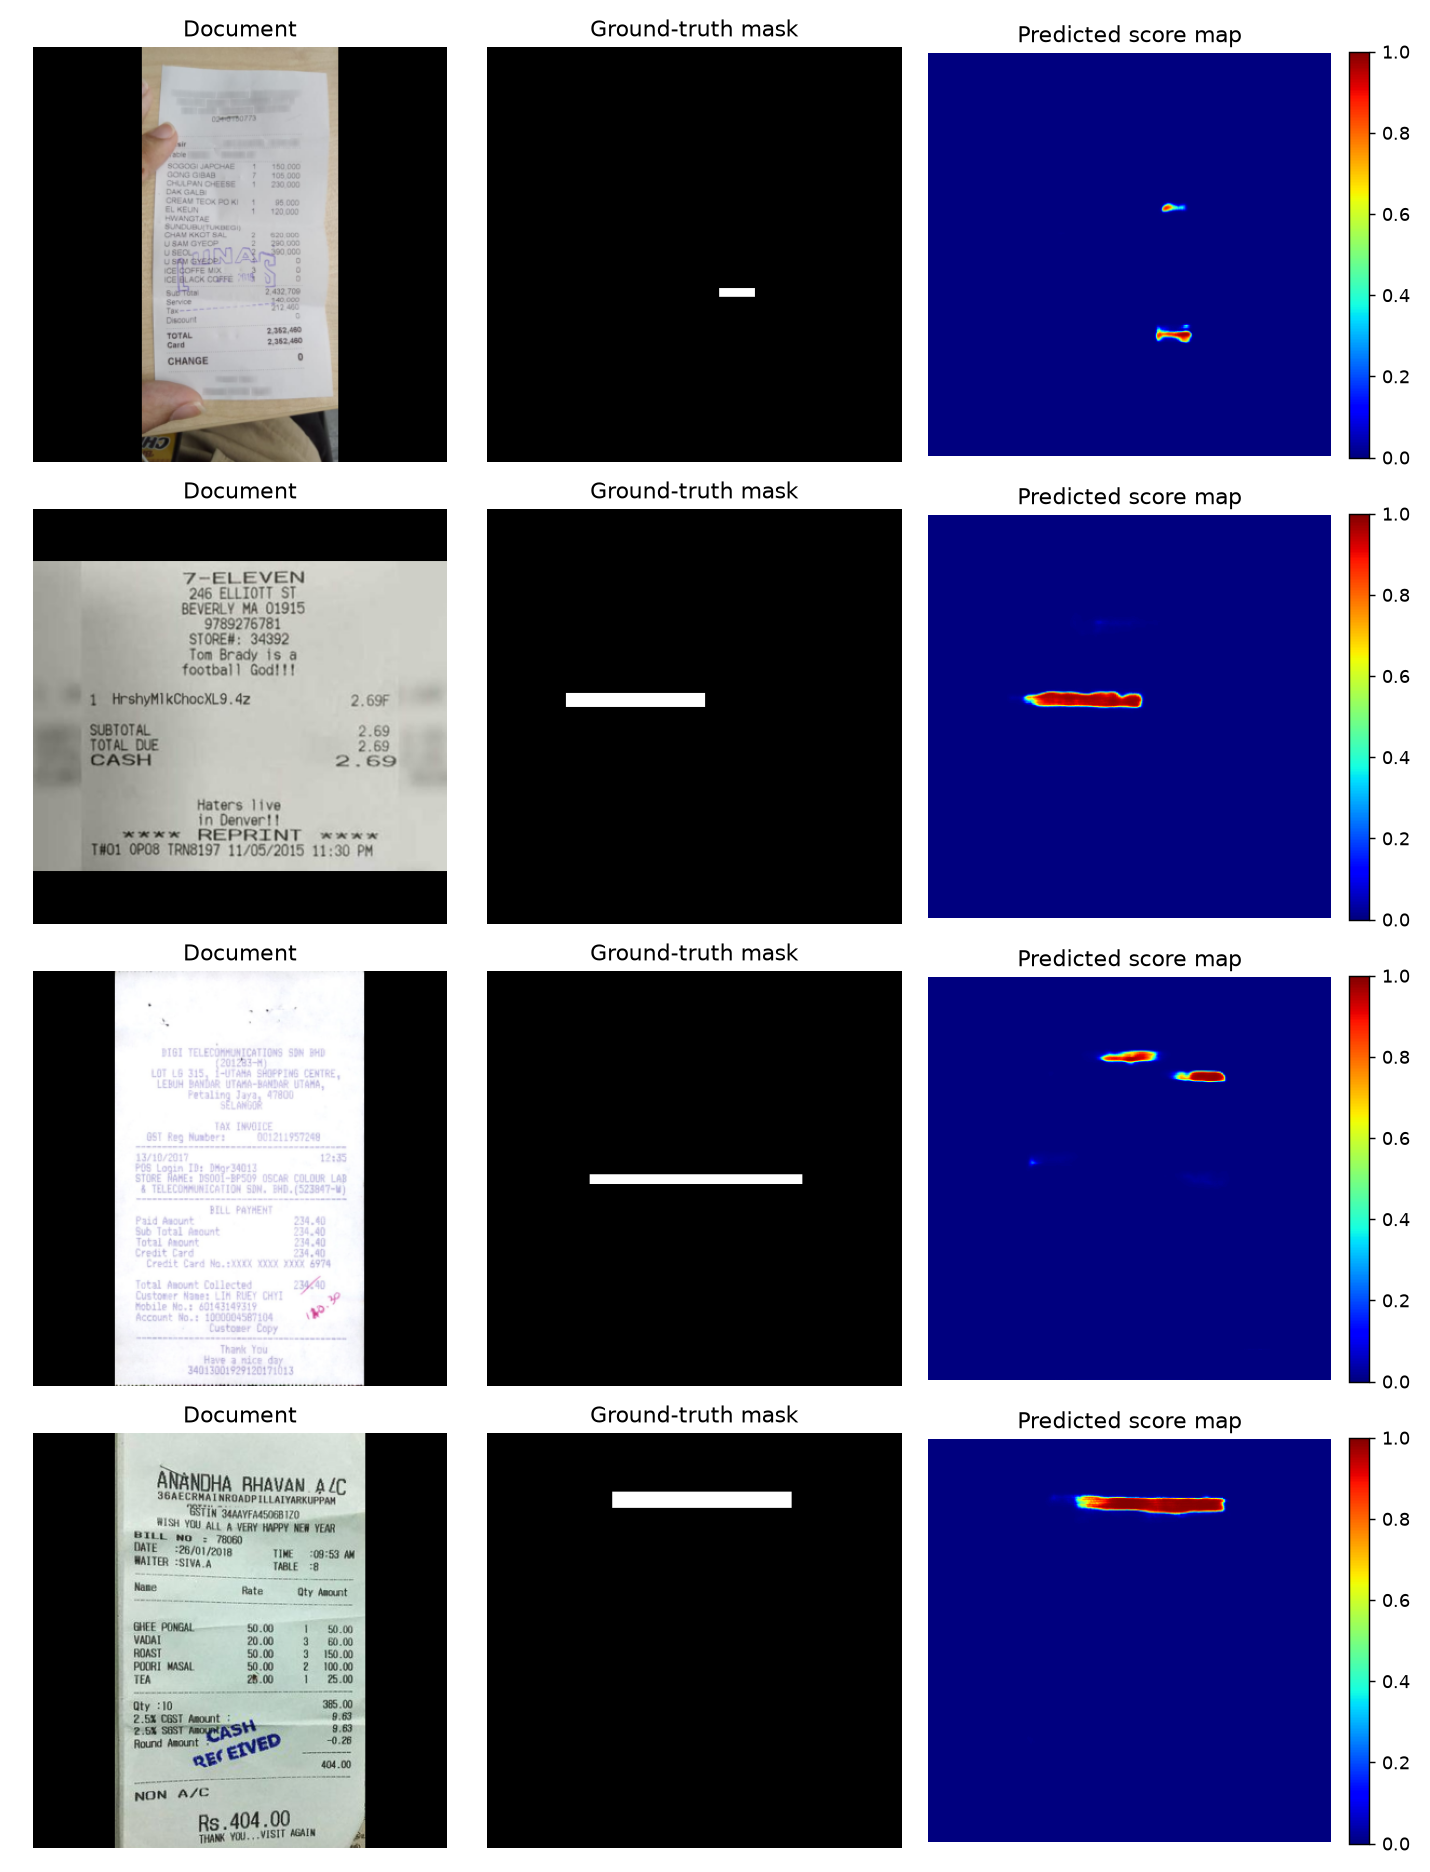
\includegraphics[width=\linewidth,keepaspectratio]{figures/fig_xai_adapted_gpt.png}\\(b)
\end{minipage}\hfill
\begin{minipage}[t]{0.31\textwidth}\centering
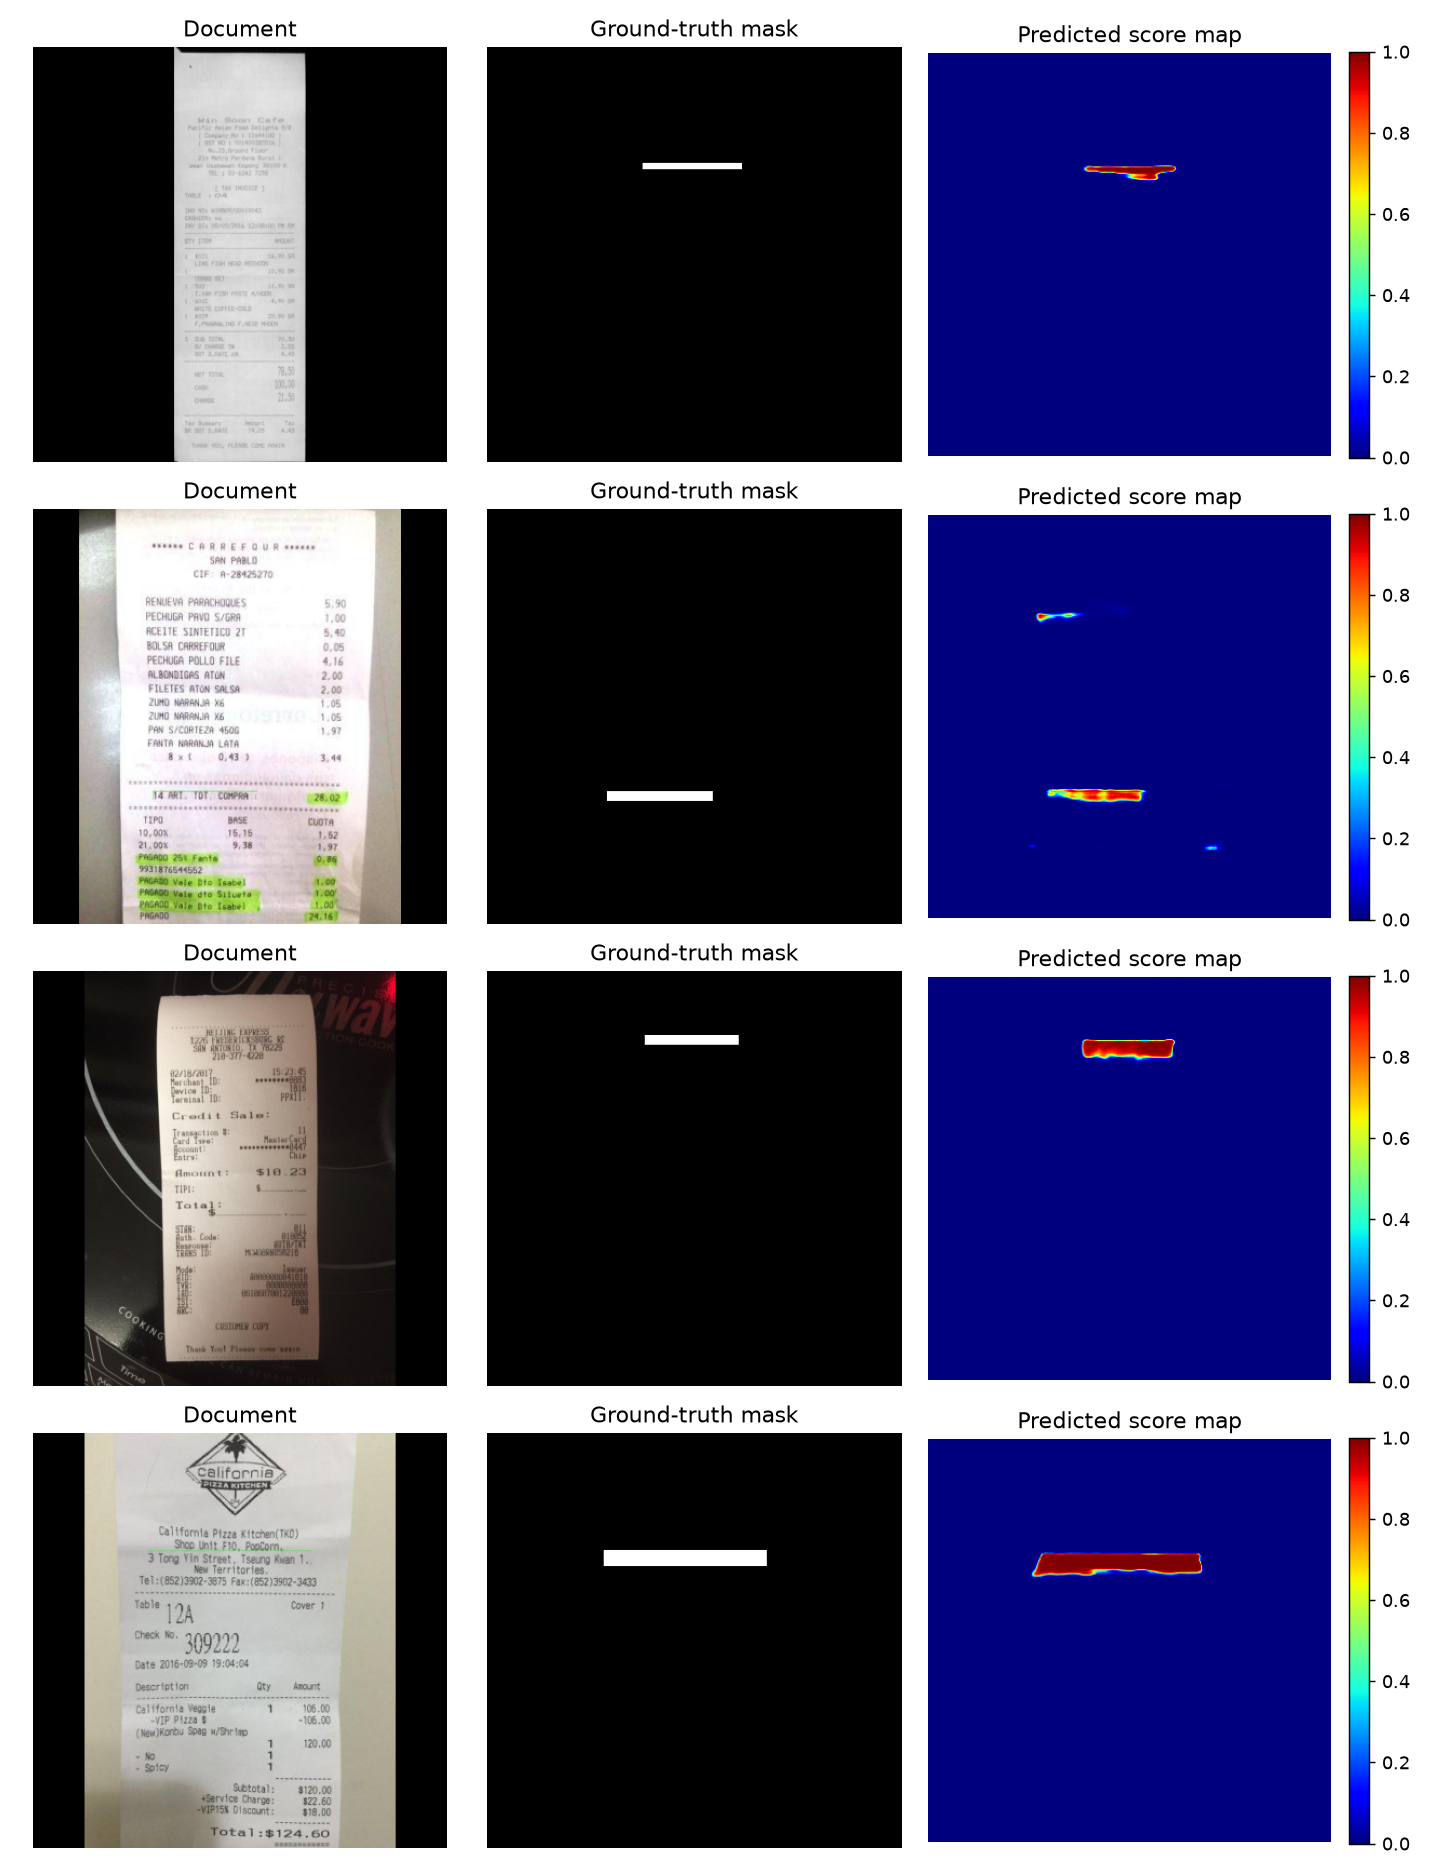
\includegraphics[width=\linewidth,keepaspectratio]{figures/fig_xai_in_domain.png}\\(c)
\end{minipage}
\caption{Predicted score maps for the same GPT-Image-2 forged documents. (a)~Zero-shot detector: diffuse and often off-target. (b)~After few-shot adaptation ($k=100$): concentrated on the edited field. (c)~In-domain Gemini: sharp and closely matching the ground truth.}
\label{fig:qual}
\end{figure}

\subsection{Where does localization fail?}\label{where-does-localization-fail}

We break down per-image IoU by document source and by tampered-area bucket on GPT-Image-2 and on in-domain Gemini (Tables~\ref{tab:source} and~\ref{tab:area}).

{
\tabcaption{Per-image IoU by document source on GPT-Image-2 and in-domain Gemini.}\label{tab:source}
\begin{longtable}[]{@{}llll@{}}
\toprule\noalign{}
Source & Standard (GPT) & Replay (GPT) & In-domain (Gemini) \\
\midrule\noalign{}
\endhead
\bottomrule\noalign{}
\endlastfoot
CORD (price fields) & \textbf{0.251} & 0.195 & 0.489 \\
WildReceipt & 0.151 & 0.092 & 0.568 \\
SROIE & 0.107 & 0.059 & 0.575 \\
XFUND (multilingual forms) & \textbf{0.013} & 0.010 & 0.372 \\
\end{longtable}
}

{
\tabcaption{Per-image IoU by tampered-area bucket.}\label{tab:area}
\begin{longtable}[]{@{}lll@{}}
\toprule\noalign{}
Tampered area & Standard (GPT) & In-domain (Gemini) \\
\midrule\noalign{}
\endhead
\bottomrule\noalign{}
\endlastfoot
\textless0.5\% & 0.170 & 0.413 \\
0.5--1\% & 0.131 & 0.572 \\
1--2\% & 0.160 & 0.619 \\
\textgreater2\% & 0.189 & 0.577 \\
\end{longtable}
}

Two findings stand out. First, cross-generator localization is \textbf{strongly source-dependent}: CORD price fields are the easiest, whereas XFUND multilingual forms are almost entirely missed. Second, in-domain performance improves with tampered-area size, but under generator shift the area effect is weak and non-monotonic. This indicates that the failure is not merely due to tiny regions; \textbf{document type, language, and layout} are major factors. Replay slightly reduces target performance across all sources, consistent with the trade-off reported in Section 6.4.

\subsection{Text-Localized High-Resolution Search (TL-HRS)}\label{text-localized-high-resolution-search-tl-hrs-1}

The full-image detector predicts at a letterboxed 384px resolution, which blurs the edited field (median tampered width $\approx$148px in the original document). A native-resolution \emph{patch segmenter} can sharpen the mask inside a 384px crop, but it still needs a crop position.

\textbf{Setup.} As described in Section 4.5, the patch segmenter is first trained on Gemini crops and then fine-tuned with the same 100 target labels used by the full-image baseline (100 GPT crops, 100 same-line negatives, 100 authentic crops, plus 100 Gemini replay crops). Used zero-shot on GPT-Image-2 it reaches only 0.459 IoU even with the oracle box; after adaptation it reaches 0.677.

\textbf{Diagnosis: the coarse stage, not the segmenter, is the bottleneck.} The natural way to position the crop is the argmax of the full-image heatmap. It fails: measured against the centre of the ground-truth field on 100 test images, the median peak error is \textbf{152 px} (0.4 crop widths; 45\% of peaks are farther than 192 px), and the 384px crop centred at the peak contains only \textbf{53\%} of the tampered pixels, versus \textbf{98\%} when centred at the true box. With the same adapted segmenter this turns a 0.65 IoU (oracle box) into 0.33 IoU. Re-running the coarse model on a zoomed 768px window, on 2×2 tiles, or on a coarse-probability centroid does not help (0.29, 0.29 and 0.37): the model is only reliable at the scale it was trained on.

\textbf{Inference.} We run the adapted patch segmenter with a coarse-to-fine cascade (stride 256, $\approx$54 windows per forged document) and select the window maximising $S(w)$ (Section 4.5). Table~\ref{tab:stagewise} reports the stage-wise results; the rest of this section quantifies why the single coarse peak fails and how dense search compares with alternative positioning strategies.

{
\tabcaption{Stage-wise localization on the full 613 forged GPT-Image-2 test images.}\label{tab:stagewise}
\begin{longtable}[]{@{}lll@{}}
\toprule\noalign{}

Setup (GPT-Image-2, full forged test, 613 images)
 & 
IoU
 & 
Notes
 \\
\midrule\noalign{}
\endhead
\bottomrule\noalign{}
\endlastfoot
Full-image few-shot, k=100 & 0.195 ± 0.037 & 3 seeds (0.158 / 0.231 / 0.195) \\
Patch, zero-shot (GT box) & 0.459 & Gemini-only patch \\
\textbf{Patch, adapted (GT box)} & \textbf{0.677 ± 0.009} & same 100 labels; 3 seeds \\
Coarse peak + adapted patch & 0.321 & median peak error 152 px \\
+ centroid re-centring & 0.358 & truncation biases the centroid \\
+ 3×3 local grid around the peak & 0.400 & helps, but the peak is too far \\
\textbf{TL-HRS, dense search (stride 96)} & \textbf{0.537 ± 0.016} & 5 seeds; per-seed values in Sec. 6.8 \\
--- oracle window (upper bound of search) & 0.653 & selection loses 0.11 \\
Ideogram (unseen generator), TL-HRS & 0.284 & oracle window 0.510 \\
Ideogram, full-image detector & 0.114 & same split (422 forged) \\
\end{longtable}
}

\begin{figure}[htbp]
\centering
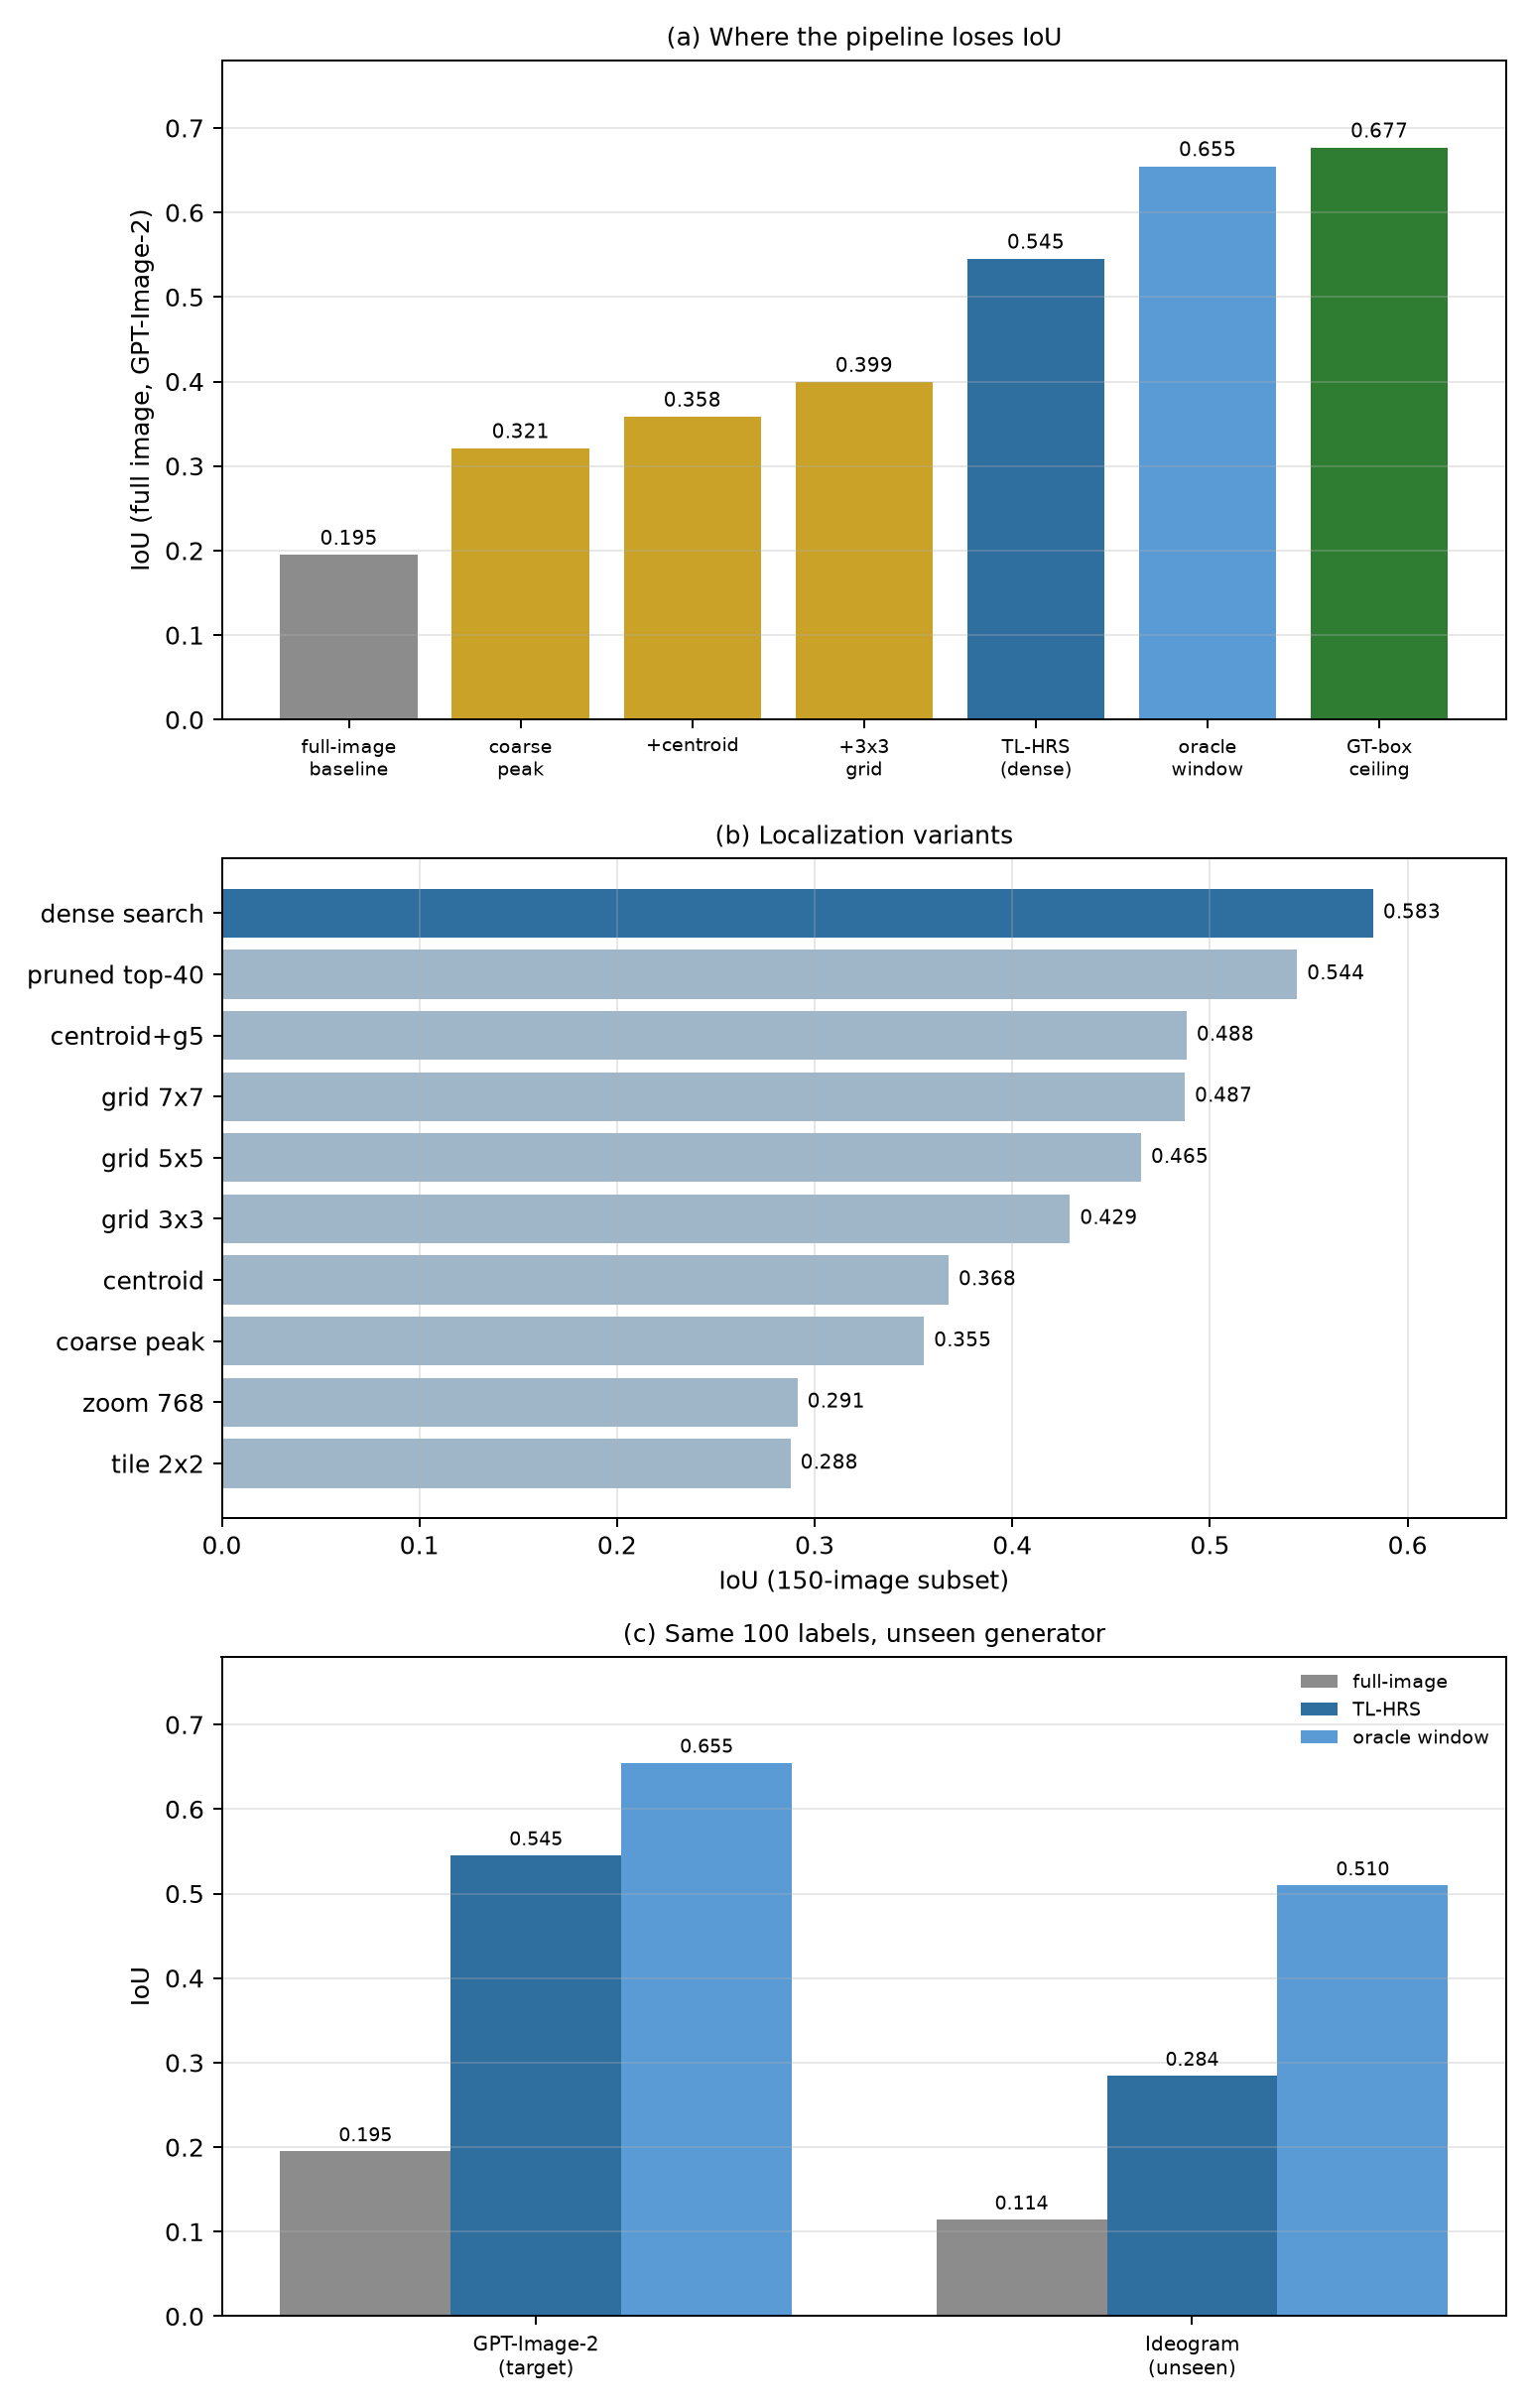
\includegraphics[width=\textwidth,height=0.85\textheight,keepaspectratio]{figures/fig_tlhrs.png}
\caption{(a)~Stage-wise IoU on the full forged test: the adapted patch alone (coarse peak) recovers little, while dense search recovers most of the oracle-window and GT-box ceilings. (b)~Localization variants on a 150-image subset: exhaustive dense search dominates centroid refinement, grids, zoom, tiling and coarse-guided pruning. (c)~The same 100 labels on the target and on a completely unseen generator.}
\label{fig:tlhrs}
\end{figure}

The headline 0.537 is the pooled IoU; the per-image mean is 0.571, with a 95\% bootstrap interval of 0.545-0.597 over 5,000 resamples. Figure~\ref{fig:tlhrs} summarizes the stage-wise and cross-generator picture. Three findings follow. \textbf{(1) Patch adaptation transfers, and the ceiling is real.} With the oracle box, the same architecture moves from 0.459 (zero-shot) to 0.677 $\pm$ 0.009 when fine-tuned with the same 100 target labels; in-domain Gemini drops only from 0.557 to 0.532, a cost that replay mitigates. \textbf{(2) The bottleneck is where to look, not what to predict.} A single coarse peak recovers only 0.321, but dense search over the same segmenter reaches 0.537 --- 2.8$\times$ the full-image baseline and 79\% of the adapted ceiling. The gap between TL-HRS and its oracle window (0.653) is entirely due to ranking the right window first. \textbf{(3) Intelligence in the search does not pay.} Coarse-guided pruning is worse than exhaustive search (top-40 windows: 0.544; top-10: 0.474; top-5: 0.431), and the coarse map is therefore not a useful prior at this resolution. Zoom, tiling and coarse centroiding are all below the single-peak-plus-grid baseline, so the simple sliding window dominates.

\textbf{6.8.1 Pre-adaptation selector study (negative results).} Before adapting the patch segmenter we tried to close the gap by improving \emph{selection} with the zero-shot patch. On the full forged test, a ResNet-18 field classifier reaches 0.193, the coarse heatmap 0.157, and the native patch response 0.158; rank fusion of all three reaches 0.199 --- none exceeds the 0.195 ± 0.037 baseline. On a 60-image subset (27 forged; it over-represents CORD and under-represents WildReceipt) we additionally tried centroid refinement, per-image MAD z-scores (monotonic, hence vacuous), line-merge, selector adaptation, and a trained DINOv2 field-vs-document-context selector (0.195); all failed. These results motivated the patch-adaptation route, and the dense search then subsumes selection: the adapted patch's own confidence, evaluated densely, is a stronger ranker than any of these learned selectors.

\textbf{6.8.2 Learned window ranker (negative result).} We test whether the gap to the oracle window (0.537 vs.~0.653) is due to a weak scoring function. We train a regressor on the same 100 target labels using nine window features --- top-1\% and top-5\% mass, max and mean probability of the predicted region, area, total mass, border contact (a cue for a truncated mask), centroid offset and compactness --- with per-image percentile normalisation, and fit both ridge regression and gradient boosting to the window's true IoU. Neither beats the simple top-1\% score (Table~\ref{tab:ranker}):

{
\tabcaption{Learned window ranker versus the top-1\% score (per-image mean IoU).}\label{tab:ranker}
\begin{longtable}[]{@{}lll@{}}
\toprule\noalign{}
Window score & GPT (150 images) & Ideogram (120 images) \\
\midrule\noalign{}
\endhead
\bottomrule\noalign{}
\endlastfoot
\textbf{top-1\% (used)} & \textbf{0.584} & \textbf{0.375} \\
Ridge (9 features) & 0.492 & 0.230 \\
GBM (9 features) & 0.583 & 0.368 \\
oracle window & 0.655 & 0.507 \\
\end{longtable}
}

The gap is therefore not a ranking-model limitation: without ground truth, several windows are genuinely indistinguishable from their features. Improving the pipeline requires a better patch detector (resolution or context), not a more expressive selector. (Numbers are per-image mean IoU on the same subsets used in Section 6.8; the Ideogram subset is easier than the full 422-image split.)

\textbf{Authentic documents.} TL-HRS is a \emph{localization} stage: it always returns a window, so it is invoked only after an image-level triage decision. In deployment we threshold the image-level score (top-1\% mean probability; Section 6.2) on the labelled authentic target samples at the operating point required by the bank's alert budget (we report 1\% FPR), and only flagged documents are passed to TL-HRS, whose $w^*$ is shown to the analyst as the suggested region. On authentic documents the triage threshold is what prevents a false alarm; the dense search itself never declares ``no forgery''. At $k=100$ the image-level AP is 0.582 and Recall@1\%FPR 0.042 (Section 6.2): a bank operating at a 1\% alert budget catches only 4\% of unseen-generator forgeries, so the triage stage, not the localizer, is the limiting factor in deployment. The low Recall@1\%FPR of the full-image detector (0.042 at $k=100$) shows that this triage is the remaining weakness, which is why we position TL-HRS as human-in-the-loop decision support rather than autonomous rejection.

\textbf{6.8.3 Label efficiency and generalization.} Adapting the patch stage is cheap: with 25 target labels the GT-box ceiling is already 0.584 (86\% of the 0.677 reached with 100), while the full-image baseline with 25 labels is 0.105. The same adapted segmenter, searched densely, transfers to Ideogram --- a generator absent from both training and adaptation --- at 0.284 IoU versus 0.114 for the full-image detector, with an oracle window of 0.510. The 0.284 -\textgreater{} 0.510 gap shows that the detector \emph{finds} the field under generator shift but its confidence is miscalibrated across generators, which is the clearest target for future work.

\subsection{Comparison with a published forensic detector}\label{comparison-with-a-published-forensic-detector}

To place TL-HRS against the literature we ran \textbf{TruFor} (CVPR 2023), a transformer + noise-fingerprint localizer trained on photographic manipulations, on the full 613 forged GPT-Image-2 images used throughout Section 6.8, with its official weights and inference script. TruFor's full-resolution attention does not fit in CPU memory for 8--35 MP documents, so we cap its input at 1024 px; every other number in this paper is at native resolution. The setting does not favour our method either: the patch detector works with 384-px crops of the same images. Table~\ref{tab:trufor} compares the two methods.

{
\tabcaption{Comparison with TruFor on the 613 forged GPT-Image-2 images.}\label{tab:trufor}
\begin{longtable}[]{@{}llll@{}}
\toprule\noalign{}

Method (613 forged GPT-Image-2)
 & 
IoU (pooled)
 & 
IoU (mean)
 & 
F1
 \\
\midrule\noalign{}
\endhead
\bottomrule\noalign{}
\endlastfoot
TruFor, threshold 0.5 & 0.018 & 0.178 & 0.035 \\
TruFor, best-F1 threshold (0.95) & 0.022 & --- & 0.042 \\
\textbf{TL-HRS (same 613 images, 5 seeds)} & \textbf{0.537 ± 0.016} & \textbf{0.571} & \textbf{0.721} \\
\end{longtable}
}

TruFor's image-level score (mean 0.63) shows that it does fire on these documents, but its localization map does not align with thin, wide text fields: pooled IoU is 0.018 and even the best threshold gives F1 0.042, whereas TL-HRS reaches 0.537 ± 0.016 on exactly the same images --- a 30× gap in pooled IoU. This is the failure mode the benchmark was built to expose --- photo-forensic localizers assume texture and noise inconsistencies at object scale, while an AI-inpainted digit is a few dozen pixels high inside a text line. We could not execute DocTamper in our environment (its mmcv build has no Windows wheel for current Python); we therefore report TruFor as the published reference and leave a full multi-detector comparison for future work.

\subsection{Accuracy--cost trade-off}\label{accuracycost-trade-off}

Dense search (stride 96) evaluates $\approx$218 windows per forged document. We test a cascade: a coarse patch scan at stride 192 proposes the top-3 windows, and each is refined on a 3×3 neighbourhood at stride 96. On the same 150-image subset this uses 66--77 windows ($\approx$3$\times$ fewer) and does not lose accuracy --- it improves slightly (Table~\ref{tab:cost}):

{
\tabcaption{Accuracy--cost trade-off of dense search versus the cascade (150-image subset).}\label{tab:cost}
\begin{longtable}[]{@{}lll@{}}
\toprule\noalign{}
Strategy & Windows / image & IoU (mean) \\
\midrule\noalign{}
\endhead
\bottomrule\noalign{}
\endlastfoot
Dense, stride 96 & 218 & 0.584 \\
\textbf{Cascade, top-1} & \textbf{66} & \textbf{0.600} \\
Cascade, top-2 & 72 & 0.607 \\
Cascade, top-3 & 77 & 0.607 \\
Oracle among visited & 77 & 0.674 \\
\end{longtable}
}

The coarse scan acts as a proposal generator and the local refinement removes the redundancy of the dense grid; at $\approx$54 windows the pipeline runs in $\approx$1.2 s per document on one consumer GPU instead of $\approx$20 s. All values are per-image mean IoU on the 150-image subset of Section 6.8.

\subsection{Cross-dataset boundary}\label{cross-dataset-boundary}

We also test zero-shot transfer to \textbf{DocTamper} (CVPR 2023), a document text-tampering benchmark with pixel masks, using the same patch detector and dense search. On its FCD split (100 images) we obtain \textbf{IoU 0.096 and F1 0.313}. The drop is expected and informative: DocTamper contains splicing and copy-move text edits rather than generative inpainting, and its authors state that it does not cover AIGC tampering. We therefore report this as a boundary condition of the method, not as evidence against it: inside the AIGC setting the model is trained for, TL-HRS reaches 0.537.

\subsection{Stride, threshold and runtime}\label{stride-threshold-and-runtime}

We sweep the coarse stride of the cascade on 60 forged test images, keeping the local refinement at stride 96, and measure wall-clock time on one consumer GPU; Table~\ref{tab:stride} reports the sweep.

{
\tabcaption{Coarse-stride sweep, threshold sensitivity and runtime (60 forged images).}\label{tab:stride}
\begin{longtable}[]{@{}llllllll@{}}
\toprule\noalign{}

coarse stride $s_1$
 & 
windows / image
 & 
time / image (s)
 & 
IoU @0.3
 & 
@0.4
 & 
@0.5
 & 
@0.6
 & 
@0.7
 \\
\midrule\noalign{}
\endhead
\bottomrule\noalign{}
\endlastfoot
128 & 147.6 & 2.85 & 0.612 & 0.615 & 0.616 & 0.614 & 0.611 \\
192 & 74.5 & 1.55 & 0.599 & 0.603 & 0.602 & 0.601 & 0.598 \\
\textbf{256} & \textbf{54.6} & \textbf{1.18} & 0.614 & \textbf{0.619} & \textbf{0.619} & 0.618 & 0.615 \\
\end{longtable}
}

Stride 256 is both the fastest (1.18 s per document, 54 windows) and the most accurate, and the IoU is flat between thresholds 0.4 and 0.6 (variation \textless{} 0.005), so the operating point is not cherry-picked.

\textbf{Image-level conformal triage fails (negative result).} Calibrating a split-conformal threshold on in-domain Gemini forges (target FNR 10\%) and deploying it on GPT-Image-2 gives an actual FNR of 25.4\% and an FPR of 67.7\% on authentic documents; even on the calibration split the FPR is 67\%, i.e.~the image-level score barely separates authentic from forged. Exchangeability is violated under generator shift, and, more fundamentally, the signal is too weak at image level. This is why the guarantees we target must be stated at the \emph{localization} level rather than for whole-image triage.

\subsection{Risk-controlled localization}\label{risk-controlled-localization}

We state the guarantee where the signal lives --- on pixels and on documents --- using Conformal Risk Control (CRC), and we keep the two losses separate. For a threshold $\lambda$, $L_i^{\mathrm{img}}(\lambda)=\mathbf{1}[s_i\le\lambda]$ is the image-level loss on forged document $i$ (the document is missed entirely), and $L_i^{\mathrm{pix}}(\lambda)$ is the fraction of its annotated pixels with score at most $\lambda$. We choose $\hat{\lambda}$ as the largest $\lambda$ whose corrected empirical risk, $(n/(n+1))\,(1/n)\sum_i L_i(\lambda)+1/(n+1)$, is below $\alpha$. We calibrate on $n_{\mathrm{cal}}\in\{25,50,100,300\}$ forged documents, evaluate on the remaining $613-n_{\mathrm{cal}}$, repeat the random split 100 times, and use all 613 authentic documents only to measure the false-positive rate. The score is the cascade score $S(w^*)$ of Section 6.8; a document is caught when $s_i>\hat{\lambda}$.

CRC bounds the loss it is given. It says nothing about false alarms, and under class imbalance and generator shift the two sides can diverge sharply. Table~\ref{tab:crc} therefore reports both.

{
\tabcaption{Conformal risk control: image- and pixel-level FNR/FPR over 100 random calibration/test splits.}\label{tab:crc}
\begin{longtable}[]{@{}llllll@{}}
\toprule\noalign{}
$\alpha$ & $n_{\mathrm{cal}}$ & image FNR (\%) & image FPR (\%) & pixel FNR (\%) & pixel FPR (\%) \\
\midrule\noalign{}
\endhead
\bottomrule\noalign{}
\endlastfoot
0.10 & 25 & 7.0 $\pm$ 5.1 & 64.9 $\pm$ 14.2 & 15.3 $\pm$ 0.5 & 5.5 \\
0.10 & 50 & 9.2 $\pm$ 4.1 & 57.8 $\pm$ 10.7 & 15.5 $\pm$ 1.1 & 5.5 \\
0.10 & 100 & 9.8 $\pm$ 3.5 & 56.0 $\pm$ 8.4 & 15.3 $\pm$ 0.6 & 5.6 \\
0.10 & 300 & \textbf{9.8 $\pm$ 2.4} & 55.8 $\pm$ 4.3 & 15.5 $\pm$ 1.3 & 5.5 \\
0.15 & 25 & 11.7 $\pm$ 5.3 & 51.6 $\pm$ 12.2 & 16.7 $\pm$ 3.2 & 4.5 \\
0.15 & 50 & 14.3 $\pm$ 5.1 & 45.5 $\pm$ 10.0 & 16.3 $\pm$ 2.3 & 4.6 \\
0.15 & 100 & 14.7 $\pm$ 3.3 & 43.1 $\pm$ 5.9 & 15.8 $\pm$ 1.8 & 5.0 \\
0.15 & 300 & 14.9 $\pm$ 2.5 & 42.1 $\pm$ 2.7 & 15.5 $\pm$ 1.3 & 5.6 \\
\end{longtable}
}

The image-level guarantee is valid but one-sided. With $n_{\mathrm{cal}}=300$, the miss rate is 9.8 $\pm$ 2.4\% at $\alpha=0.10$ and 14.9 $\pm$ 2.5\% at $\alpha=0.15$: the construction does what it promises, and the observed risk approaches $\alpha$ from below as $n_{\mathrm{cal}}$ grows (7.0\% at $n_{\mathrm{cal}}=25$), because with few calibration documents $\hat{\lambda}$ is fitted to a noisy empirical risk and under-covers. The same thresholds, however, flag 55.8 $\pm$ 4.3\% ($\alpha=0.10$) and 42.1 $\pm$ 2.7\% ($\alpha=0.15$) of authentic documents. A bank that insists on missing at most 10\% of forgeries would send more than half of all genuine documents to manual review.

This does not mean that the cascade score is useless for triage. Relative to the full-image score it is a much better ranker: image AUC 0.825 versus 0.565, image AP 0.845 versus 0.582, and Recall@1\%FPR 0.286 versus 0.042, a 6.8$\times$ gain. But a 6.8$\times$ improvement over a near-random ranker is not a solution: at the 1\% alert budget 71\% of forgeries still pass unreviewed, and the conformal threshold that bounds the miss rate at 10\% operates at 56\% FPR. We therefore do not claim that TL-HRS restores image-level triage. The score used for localization is a better ranking signal, but triage remains the deployment bottleneck.

At pixel level the picture is different. FNR is 15.3--16.7\% across all settings at 4.5--5.6\% pixel FPR, and moving $\alpha$ from 0.10 to 0.15 barely changes it because a structural floor dominates: in about 15\% of forged documents the selected window $w^*$ does not cover the whole annotation, and those pixels are false negatives at every threshold. No calibrator can go below this window-miss floor, so the nominal 10\% pixel guarantee is not met and $\alpha=0.15$ is met only marginally at $n_{\mathrm{cal}}=300$ (15.5 $\pm$ 1.3\%). The low pixel FPR is a consequence of sparsity (masks cover $\approx$1\% of the pixels): even a permissive threshold adds few false positives relative to background. Certifying a 10\% pixel-level FNR requires better window selection or a finer segmenter, not a different calibration. We report these numbers as measured rather than tuning $\lambda$ to a favourable value.

The replay ablation at the TL-HRS level (IoU pooled / mean; Table~\ref{tab:replay}) shows that replay helps on every split, so it is not a target/source trade-off at this layer:

{
\tabcaption{Replay ablation at the TL-HRS level (IoU pooled / mean).}\label{tab:replay}
\begin{longtable}[]{@{}llll@{}}
\toprule\noalign{}

 & 
GPT (target adapted)
 & 
Gemini (source retention)
 & 
Ideogram (unseen)
 \\
\midrule\noalign{}
\endhead
\bottomrule\noalign{}
\endlastfoot
Replay 100 & \textbf{0.564 / 0.590} & \textbf{0.469 / 0.701} & \textbf{0.278 / 0.381} \\
No replay & 0.523 / 0.574 & 0.449 / 0.658 & 0.226 / 0.323 \\
\end{longtable}
}

\textbf{Full-test cascade and image-level triage.} Running the cascade (stride 256) over all 1,226 GPT-Image-2 test images (613 forged + 613 authentic) takes 1.04 s per image and gives IoU 0.564 pooled / 0.590 mean, F1 0.721 pooled. Using the same score S(w*) for whole-image triage is substantially better than the full-image detector: image AUC 0.825 versus 0.565, image AP 0.845 versus 0.582, and \textbf{Recall@1\%FPR 0.286 versus 0.042} (a 6.8x gain). This is a better ranking signal, not a solved triage stage: at a 1\% alert budget 71\% of forgeries are still missed, and the conformal operating point that bounds the miss rate at 10\% flags 56\% of authentic documents. The localization stage therefore improves triage but does not fix it.

\subsection{Robustness to post-processing}\label{robustness-to-post-processing}

A forged document rarely reaches the bank as a pristine PNG: it is screenshotted, recompressed, or resized on its way. We therefore re-run the cascade on a fixed subset of 200 forged and 100 authentic GPT-Image-2 documents under four corruptions: JPEG quality 90 and 75, a $0.75\times$ downsample followed by bilinear upsampling, and Gaussian blur ($5\times5$, $\sigma{=}1$). We compare the baseline patch adapter of Section 6.8 with a variant fine-tuned with the same 100 labels plus random JPEG augmentation (quality 50--95 applied to 50\% of patch crops); this is the only difference between the two runs. The subset is the first 200/100 documents of the fixed test list and is easier than the full split (pooled IoU 0.705 without corruption for the baseline versus 0.564 in Table~\ref{tab:stagewise}); absolute values are therefore not comparable across tables, and we read Table~\ref{tab:robust} only as relative retention. With 100 authentic documents the 1\% FPR operating point is empirical and coarse (about one false positive), so Recall@1\%FPR is quantized in steps of 0.005.

{
\tabcaption{Robustness of the cascade to post-processing on a fixed subset of 200 forged and 100 authentic GPT-Image-2 documents, for the baseline patch adapter and for a variant trained with JPEG augmentation on the same 100 labels. All rows use the same documents; only relative comparisons within the table are meaningful.}\label{tab:robust}
\begin{longtable}[]{@{}lrrrrrr@{}}
\toprule\noalign{}
Corruption & IoU (pooled) & IoU (mean) & F1 & Image AUC & Image AP & Recall@1\%FPR \\
\midrule\noalign{}
\endhead
\bottomrule\noalign{}
\endlastfoot
\multicolumn{7}{l}{\textit{Baseline patch adapter (no compression augmentation)}} \\
None & 0.705 & 0.725 & 0.827 & 0.908 & 0.953 & 0.520 \\
JPEG q90 & 0.214 & 0.278 & 0.352 & 0.541 & 0.718 & 0.070 \\
JPEG q75 & 0.081 & 0.117 & 0.149 & 0.397 & 0.594 & 0.005 \\
Resize $0.75\times$ & 0.629 & 0.655 & 0.772 & 0.815 & 0.903 & 0.305 \\
Blur $\sigma{=}1$ & 0.579 & 0.617 & 0.733 & 0.778 & 0.882 & 0.240 \\
\midrule
\multicolumn{7}{l}{\textit{+ JPEG augmentation during patch adaptation}} \\
None & 0.621 & 0.641 & 0.766 & 0.807 & 0.904 & 0.345 \\
JPEG q90 & 0.512 & 0.531 & 0.678 & 0.669 & 0.822 & 0.165 \\
JPEG q75 & 0.449 & 0.482 & 0.620 & 0.623 & 0.786 & 0.130 \\
Resize $0.75\times$ & 0.505 & 0.553 & 0.671 & 0.733 & 0.854 & 0.225 \\
Blur $\sigma{=}1$ & 0.476 & 0.544 & 0.645 & 0.724 & 0.850 & 0.205 \\
\end{longtable}
}

Three observations follow. \textbf{(1) Without compression augmentation, JPEG is catastrophic.} Quality 90 reduces pooled IoU from 0.705 to 0.214 (30\% retained) and Recall@1\%FPR from 0.520 to 0.070; quality 75 leaves 0.081 IoU, 0.149 F1 and 0.005 Recall@1\%FPR, and image AUC falls to 0.397, below chance on this subset. This is consistent with the detector relying on high-frequency generator traces that quantization removes, and it matters operationally because recompression is ubiquitous. We report the below-chance AUC as measured; with 200 forged documents it is also the noisiest cell in the table. \textbf{(2) JPEG augmentation removes most of that loss.} Under the same 100 labels and replay budget, quality 90 improves from 0.214 to 0.512 pooled IoU and quality 75 from 0.081 to 0.449 (72\% of the augmented model's own clean 0.621); image AUC rises from 0.541/0.397 to 0.669/0.623, and Recall@1\%FPR at quality 75 rises from 0.005 to 0.130. \textbf{(3) The gain is targeted and not free.} The augmented model pays on clean documents (0.705 $\rightarrow$ 0.621 pooled IoU; Recall@1\%FPR 0.520 $\rightarrow$ 0.345) and on the two corruptions it was not trained for (resize 0.629 $\rightarrow$ 0.505; blur 0.579 $\rightarrow$ 0.476). Matching augmentation to the ingestion pipeline therefore matters more than adding it blindly. Even with augmentation, quality 75 still loses 28\% of the clean IoU and triage at 1\% FPR catches 13\% of forgeries versus 34.5\% clean, so the gap is narrowed but not closed. Ranking and localization degrade together, so recalibration cannot recover the lost IoU.

\bigskip


\section{Backbone generality}
To check that the findings are not an artefact of ResNet-18, we repeat the pipeline with SegFormer-B2 (ImageNet pre-training, the same Gemini training recipe, the same 100 GPT labels and the same cascade).

\begin{table}[H]\centering\small
\begin{tabular}{lccccccc}
\toprule
Backbone & GT-box & IoU pooled/mean & F1 & Img AUC & Img AP & R@1\% & s/img \\
\midrule
ResNet-18 & 0.677 & 0.564 / 0.590 & 0.721 & 0.825 & 0.845 & 0.286 & 1.04 \\
SegFormer-B2 & \textbf{0.776} & \textbf{0.658} / \textbf{0.670} & \textbf{0.794} & \textbf{0.891} & \textbf{0.911} & \textbf{0.527} & 2.44 \\
\bottomrule
\end{tabular}
\end{table}

SegFormer-B2 improves every metric: the ceiling rises from 0.677 to 0.776, the automatic IoU from 0.564 to 0.658 (3.4x the full-image baseline, 85\% of its ceiling), and Recall@1\%FPR from 0.286 to 0.527, at 2.4\,s instead of 1.0\,s per document. The phenomenon is backbone-agnostic, and the transformer is the better deployment choice when latency allows.

\section{Discussion}\label{discussion}

\textbf{Why does adaptation help?} Fine-tuning on a few target samples appears to sharpen the spatial response around the edited region, rather than merely shifting a global threshold. This is consistent with the high pixel AUC before adaptation and with the failure of threshold-calibration methods.

\textbf{Why does forgetting happen?} The base detector's features encode generator-specific artefacts. Fine-tuning on a new generator overwrites part of this encoding. Rehearsal of a small number of old samples anchors the old decision boundary and restores in-domain performance.

\textbf{Why do calibration and selection fail?} Calibration is generator-specific and does not change pixel ranking; sample selection does not address the underlying localization error. These negative results are useful: they rule out several intuitive but ineffective remedies. They also show that \emph{learned} selectors trained on a handful of target images overfit the wrong cues; the adapted patch's own dense confidence is a better ranker.

\textbf{Where is the ceiling, and what limits us?} Adapting the patch segmenter with the same 100 target labels raises the oracle-box ceiling from 0.459 to 0.677, so segmentation is no longer the wall. The wall is \emph{where to look}: the full-image peak is 152 px (median) from the field centre, and the crop it defines covers only half of the tampered pixels. Dense high-resolution search removes the dependence on that peak and reaches 0.537 ± 0.016 (79\% of the ceiling). The remaining gap splits into two measured quantities: 0.537 -\textgreater{} 0.653 is window \emph{ranking} (oracle window), and 0.653 -\textgreater{} 0.677 is the residual crop/segmentation limit. Under generator shift the ranking gap widens (0.284 observed vs.~0.510 oracle on Ideogram), which points to confidence calibration across generators rather than to a weaker detector.

\bigskip

\section{Limitations}\label{limitations}

\begin{itemize}
\tightlist
\item
  \textbf{Small, narrow benchmark.} AIForge-Doc contains $\approx$4k forged receipts/forms; generalization to other document types, languages, and bank-specific data is unverified.
\item
  \textbf{Three generators.} Gemini, Ideogram, and GPT-Image-2 do not cover the full space of generative editors.
\item
  \textbf{Synthetic edits.} Forgeries replace a single numeric field; whole-document synthesis and signature forgery are out of scope.
\item
\textbf{Two backbones.} We evaluate ResNet-18 and SegFormer-B2; larger or text-aware models may behave differently, but the trend is consistent across the two.
\item
  \textbf{Modest full-image performance.} The full-image detector remains modest after adaptation (0.195 ± 0.037); the TL-HRS stage reaches 0.537 ± 0.016, and the remaining gap to its 0.677 adapted ceiling is split between window ranking (0.653) and the crop limit.
\item
  \textbf{Inference cost.} The cascade runs $\approx$54 window passes per forged document ($\approx$1.2 s on one consumer GPU). This is acceptable for offline forensic review but not for high-throughput streaming; coarse-guided pruning currently costs 0.011 IoU or more.
\item
  \textbf{Generator-shift ranking gap.} On Ideogram the detector's oracle window is 0.510 but the selected window scores 0.284, so confidence is miscalibrated across generators.
\item
  \textbf{Single published baseline.} We compare against TruFor only, on the full 613 forged test images (capped at 1024 px because of CPU memory); DocTamper could not be built in our environment, so a multi-detector comparison remains future work.
\item
  \textbf{Post-processing.} JPEG recompression at quality 75 removes most of the signal without compression augmentation (Section~\ref{robustness-to-post-processing}); augmenting the patch adapter restores 72\% of its clean IoU under q75 but costs clean accuracy and does not help resize or blur.
\item
  \textbf{Variance.} Results vary across seeds; we report mean ± std over three seeds for all headline numbers.
\end{itemize}

\bigskip

\section{Future Work}\label{future-work}

A natural extension is \textbf{federated adaptation}~\cite{mcmahan2017fedavg}: when one bank encounters a new generator and collects a small labelled set, it could share the \emph{model update} (not raw customer data) with other institutions, allowing them to defend against the same threat without violating data-protection regulations. Combining few-shot adaptation with secure aggregation and differential privacy is an important direction.

Other directions include: (i) calibrating the patch confidence across generators to close the 0.284 -\textgreater{} 0.510 ranking gap on unseen generators, and scoring windows jointly rather than independently; (ii) continual adaptation over a stream of generators; (iii) stronger domain-generalization objectives; (iv) broader benchmarks across document types and languages; and (v) calibrated uncertainty for human-in-the-loop review.

\bigskip

\section{Conclusion}\label{conclusion}

We studied label-efficient adaptation of AI-forged document detectors under generator shift. A detector trained on one generator collapses on unseen generators, but a small number of labelled target samples recovers localization substantially, and a small rehearsal buffer preserves old-generator performance with negligible forgetting. Our analysis shows that the remaining bottleneck is localization precision rather than threshold calibration, and that several intuitive remedies (calibration, adaptive thresholding, sample selection, encoder freezing) do not provide consistent gains. Adapting a native-resolution patch segmenter with the same 100 labels raises the localization ceiling from 0.459 to 0.677. The coarse peak used to position that segmenter is itself the wall --- it misses the field centre by 152 px (median) and covers only 53\% of the tampered pixels --- and replacing it with dense high-resolution search yields \textbf{0.537 ± 0.016 IoU} on the full unseen generator (2.8× the full-image baseline, 79\% of the ceiling). The same pipeline reaches 0.284 IoU on a completely unseen generator (Ideogram) versus 0.114 for the full-image detector, with an oracle window of 0.510: the detector finds the field, but cross-generator confidence ranking remains the open problem. We hope these results provide a realistic foundation for deploying and adapting document-fraud detectors in banking workflows.

\bigskip

\bibliographystyle{elsarticle-num}
\bibliography{references}
\end{document}
